% Chapter Template

\chapter{Results and Comparison} % Main chapter title

\label{Chapter5} % Change X to a consecutive number; for referencing this chapter elsewhere, use \ref{ChapterX}

In this chapter, we'll talk about results, comparison between different ways of arranging the \glspl{map} and future work this project can lead to.

%----------------------------------------------------------------------------------------
%	SECTION
%----------------------------------------------------------------------------------------

\section{General Results}

For starters, this project successfully implemented the functionality of browsing through the dataset Mandelbrot set with the techniques of \gls{fpc} as shown in \gmref{fig:chap5:basic}. There is a focus view, a context view and a control panel located on the right side of the screen which can be hidden, and four different categories of controls this control panel can offer, shown in \gmref{fig:chap5:fourcate}. All of them with nice modern looks.

\begin{figure}[H]
\centering
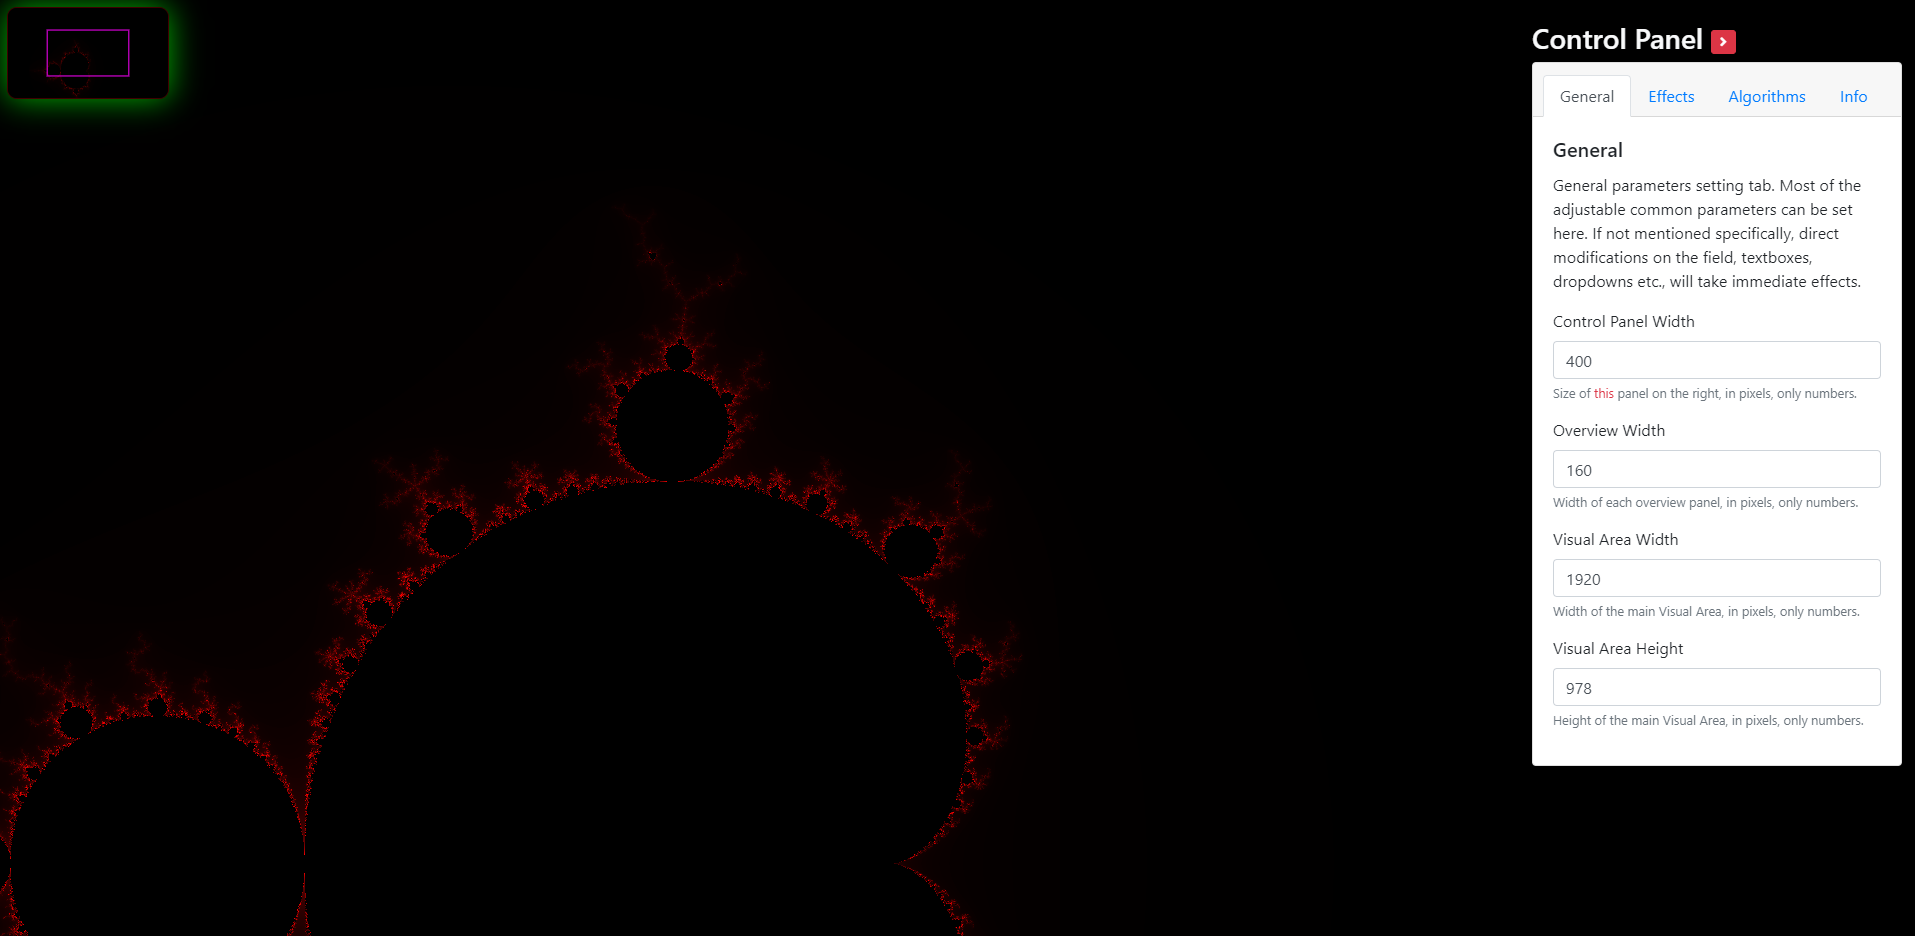
\includegraphics[width=\textwidth,keepaspectratio]{Figures/Chapter5/basic.png}
% 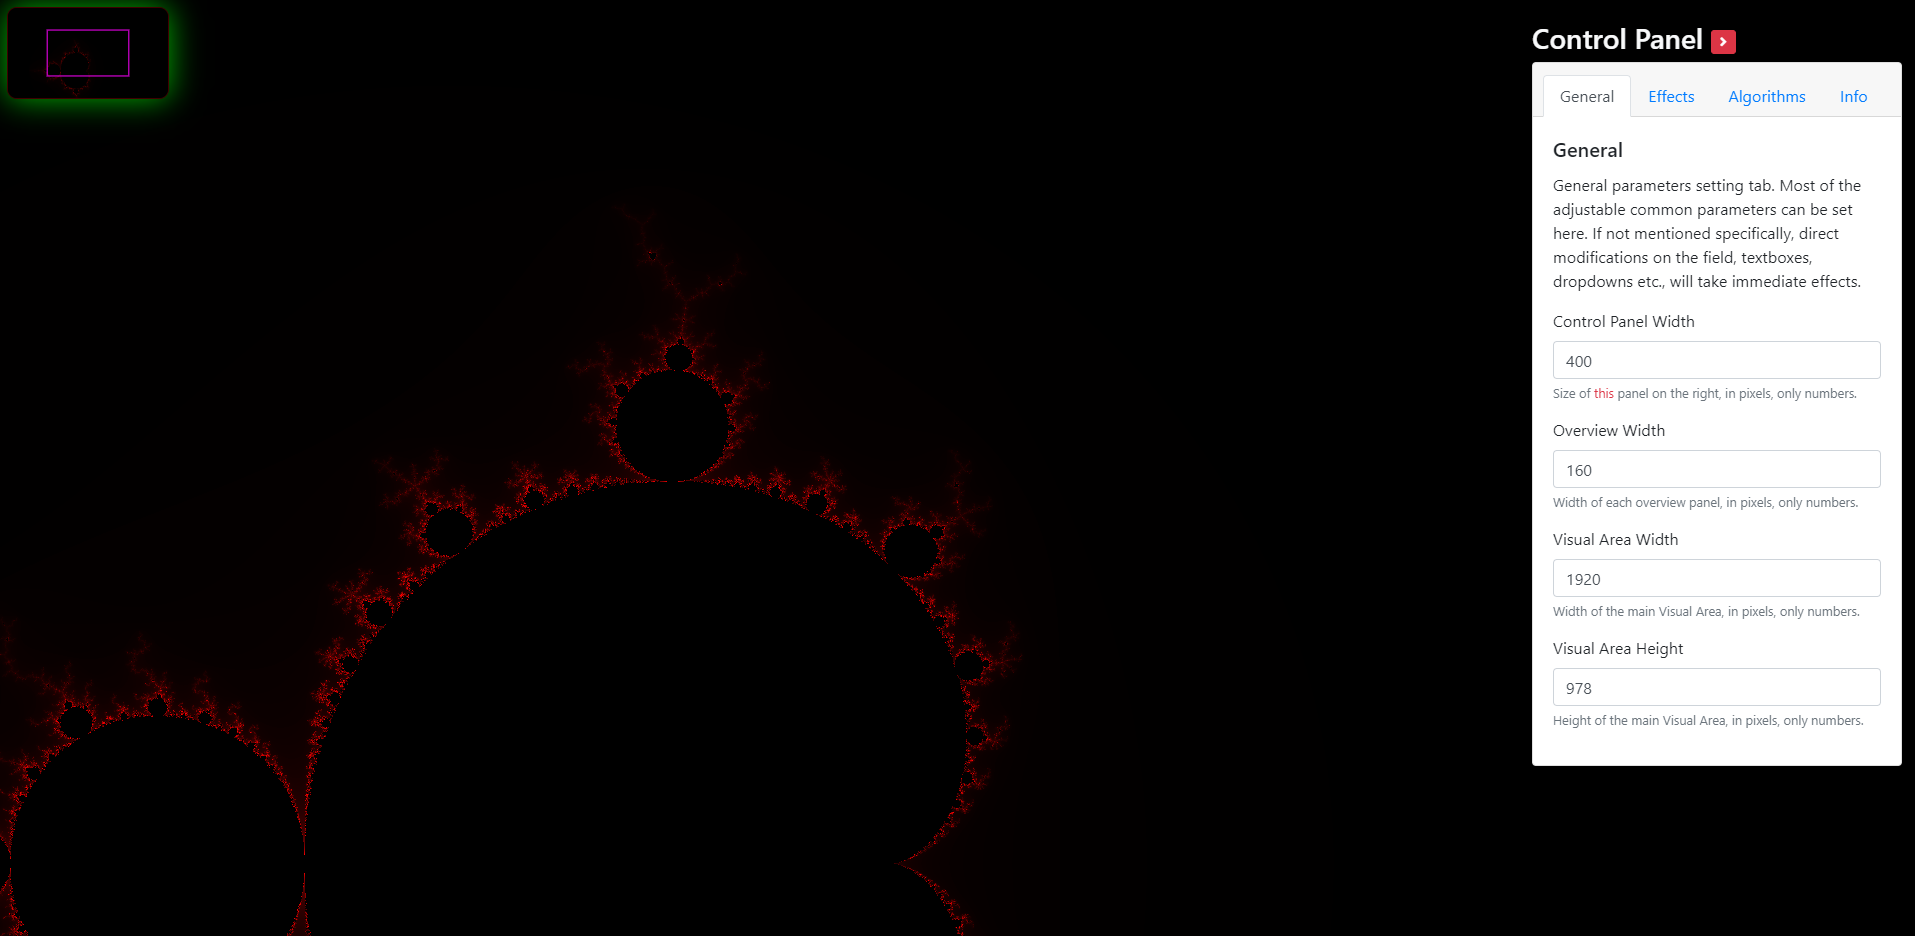
\includegraphics{Figures/Chapter5/basic.png}
\decoRule
\caption[Basic UI]{A basic \gls{ui} of the project under the resolution of \gls{fhd}. Note that the resolution is not \texttt{1920 x 1080} is because the \gls{ui} of the browser Google Chrome is occupying some slices of the \gls{fhd} screen.}
\label{fig:chap5:basic}
\end{figure}

\begin{figure}[H]
\centering
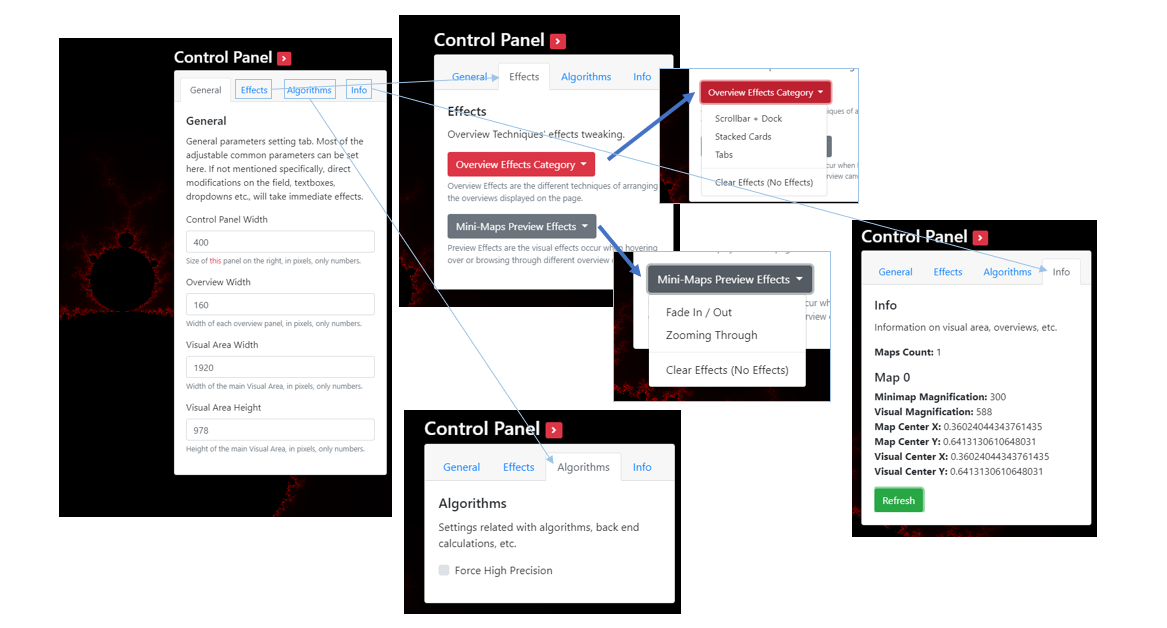
\includegraphics[width=\textwidth,keepaspectratio]{Figures/Chapter5/fourcate.png}
% 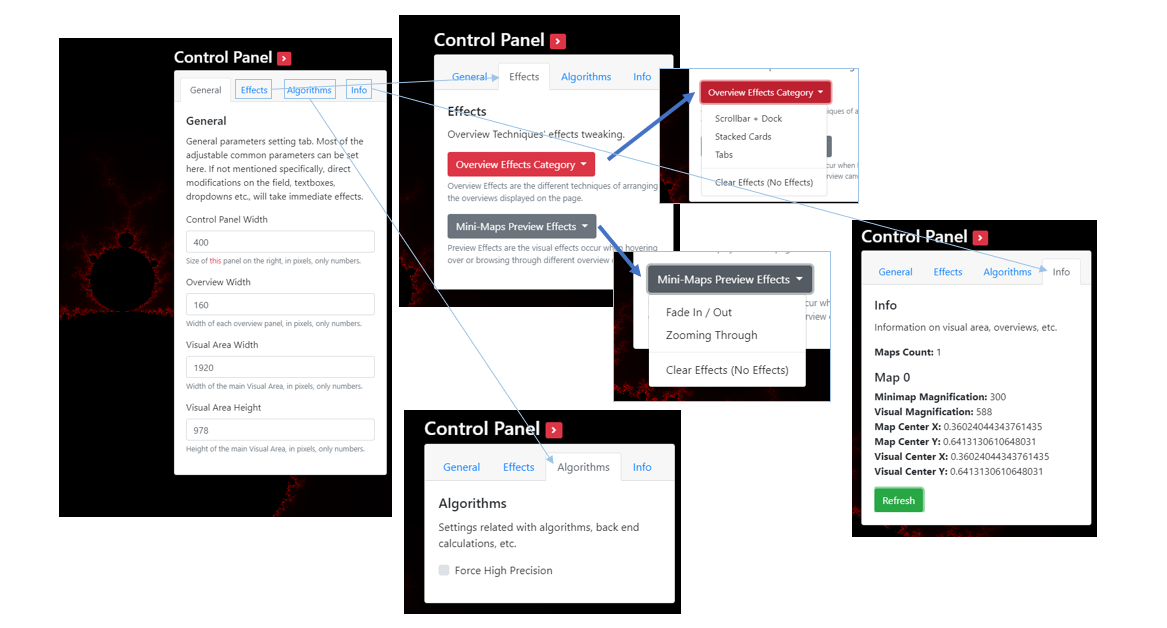
\includegraphics{Figures/Chapter5/fourcate.png}
\decoRule
\caption[The Four Categories of the Control Panel]{The four categories that the control panel offers to control the behaviour of the project in different aspects: general, effects, algorithms and info.}
\label{fig:chap5:fourcate}
\end{figure}

Other basic functionalities such as zooming and panning are also implemented, which will be described in the following sections.

\subsection{Zooming}

The zooming functionality works as expected shown in \gmref{fig:chap5:zooming}, when user scrolls the mouse wheel, the magnification level is going to increase or decrease until the user stops to scroll. When the magnification level increases or decreases, more context views is going to be created or removed based on the sizes of the projection area related with the parent context view. The later the context view shows up, the closer the context is to the focus area.

\begin{figure}[H]
\centering
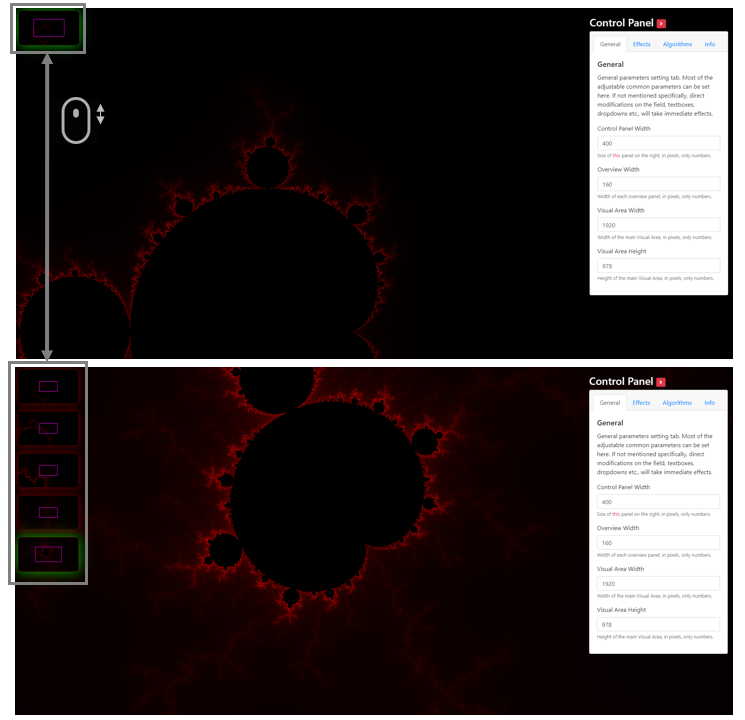
\includegraphics[width=\textwidth,keepaspectratio]{Figures/Chapter5/zooming.png}
% 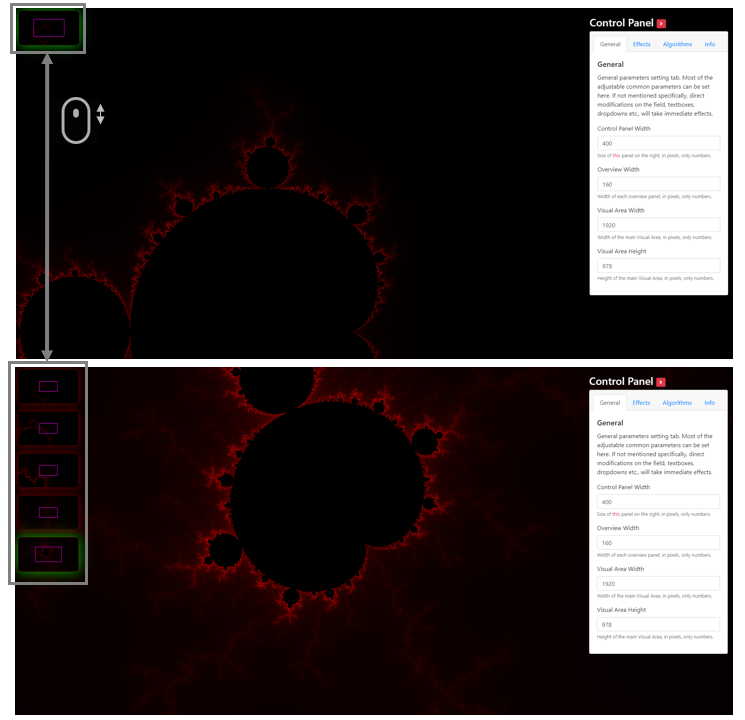
\includegraphics{Figures/Chapter5/zooming.png}
\decoRule
\caption[Zooming Functionality]{A simple illustration of the zooming functionality --- When user scrolls the mouse wheel to zoom in, more context views show up. The reverse way, zooming out, works also in a similar way.}
\label{fig:chap5:zooming}
\end{figure}

\subsection{Panning}

The panning functionality works like any map applications. When user left-clicks on point and moves the mouse the detail view is going to be pinned to the mouse cursor and ``dragged'' by it, until the user releases the left mouse button, as shown in \gmref{fig:chap5:panning}.

\begin{figure}[H]
\centering
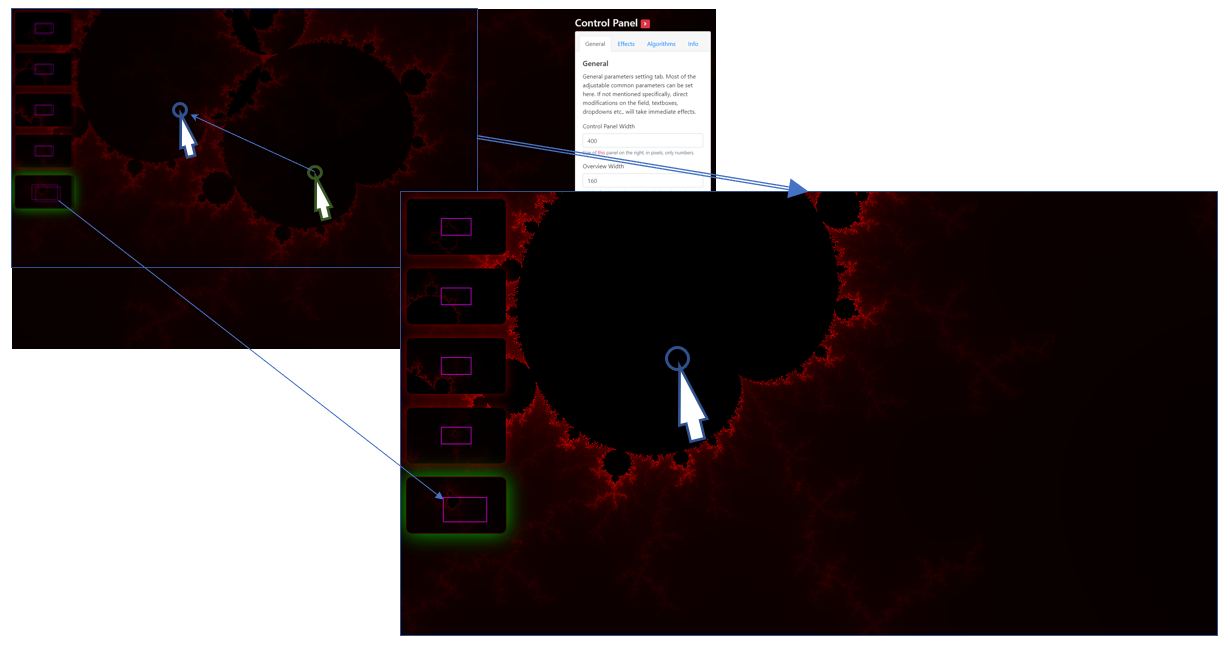
\includegraphics[width=\textwidth,keepaspectratio]{Figures/Chapter5/panning.png}
% 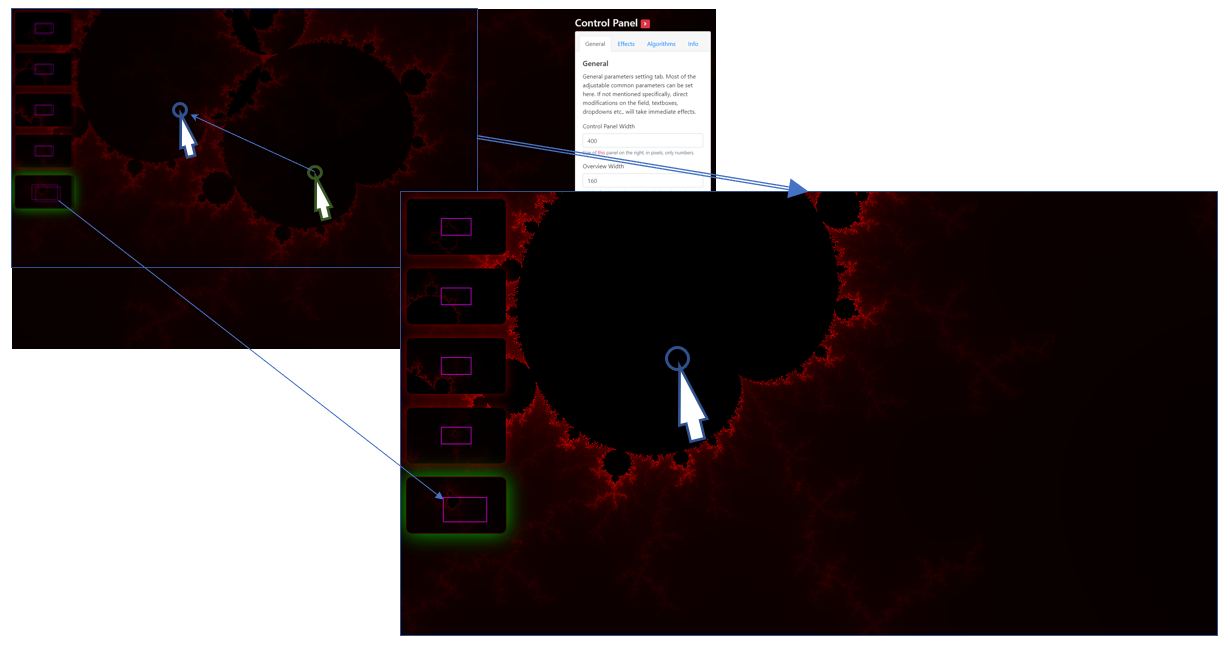
\includegraphics{Figures/Chapter5/panning.png}
\decoRule
\caption[Panning Functionality]{A simple illustration of the panning functionality --- User has the ability to drag the dataset around, left-click to start the panning and release the left mouse button to stop it when desired.}
\label{fig:chap5:panning}
\end{figure}

\subsection{Buffering That Does Not Block UI}

During the process of front end -- back end communication, the dataset calculation doesn't block the front end \gls{ui} from hanging, as shown in \gmref{fig:chap5:buffer}. When a certain part of dataset is resolved and the time passed exceeds $500$ milliseconds, this part of data is immediately transfered and rendered on the corresponding views. There is also a warning color halo being displayed around the context views that's still waiting for complete data.

\begin{figure}[H]
\centering
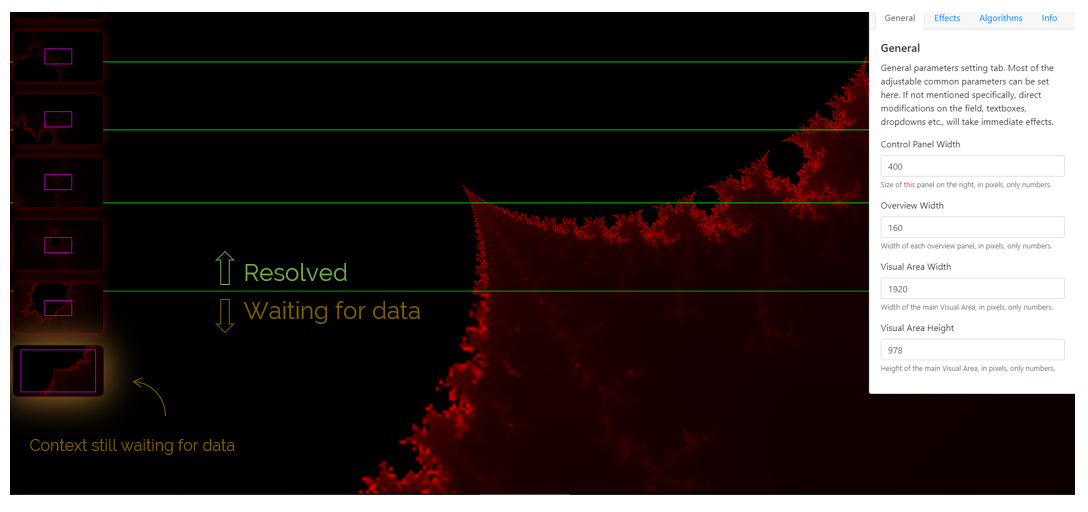
\includegraphics[width=\textwidth,keepaspectratio]{Figures/Chapter5/buffer.png}
% 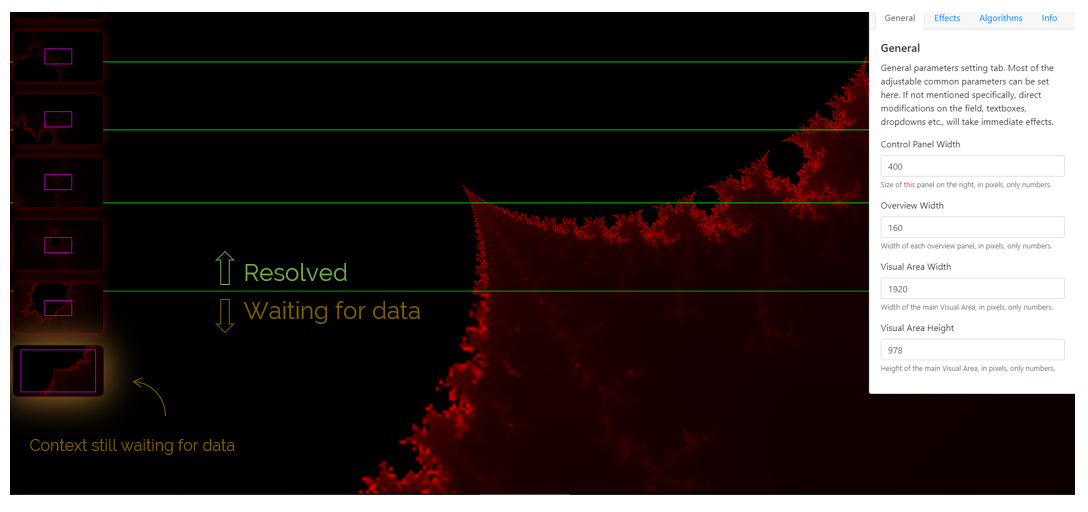
\includegraphics{Figures/Chapter5/buffer.png}
\decoRule
\caption[Data Resolving Buffering]{When the back end is trying to resolve a certain part of the dataset, the front end can be operated on as usual. The green blocks in the detail view indicates the area that just got resolved and the other part of the detail view, as can be seen a little bit blurry, are still yet to be resolved.}
\label{fig:chap5:buffer}
\end{figure}

\subsection{Deeper Into the Dataset}

The implemented application in this project can go deep into the dataset efficiently, as shown in \gmref{fig:chap5:deep}. Under the normal settings, as no management of the context views is applied, they occupy quite a bit of the visual area. The illustration shown in \gmref{fig:chap5:deep} has a magnification level of $\textbf{62,458,965,053,016}$ and took only around $5$ seconds to finish the complete rendering.

\begin{figure}[H]
\centering
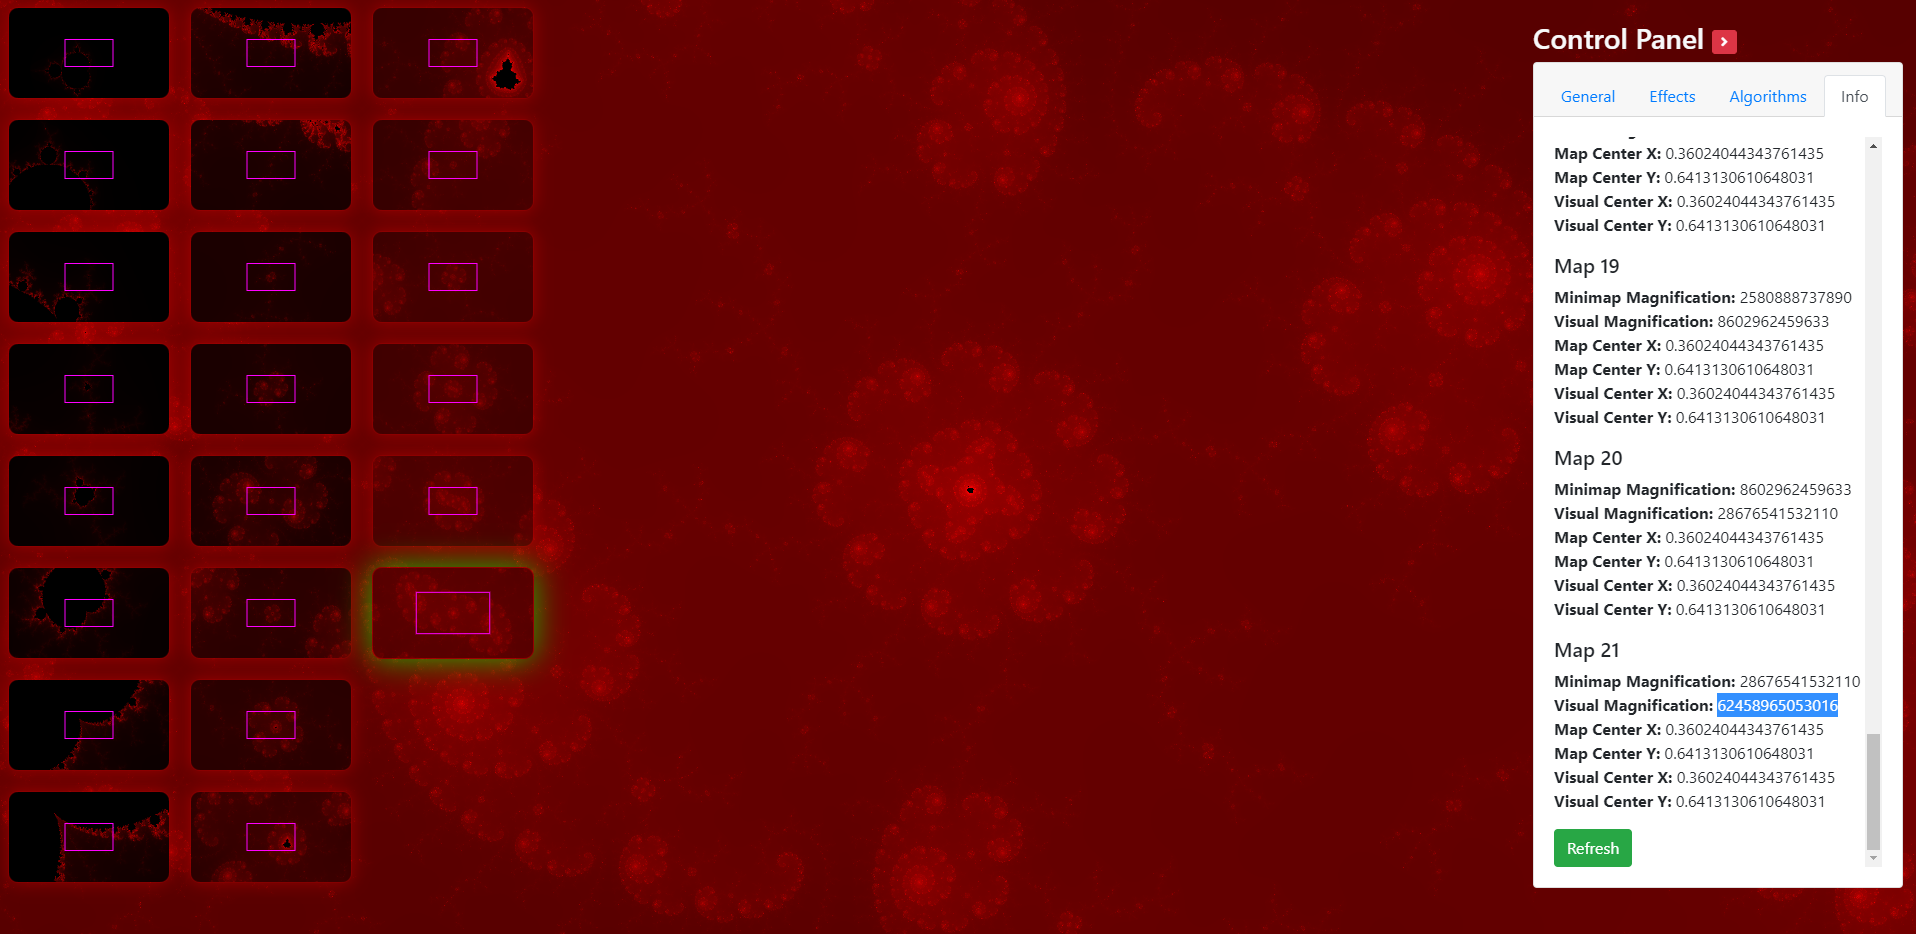
\includegraphics[width=\textwidth,keepaspectratio]{Figures/Chapter5/deep.png}
% 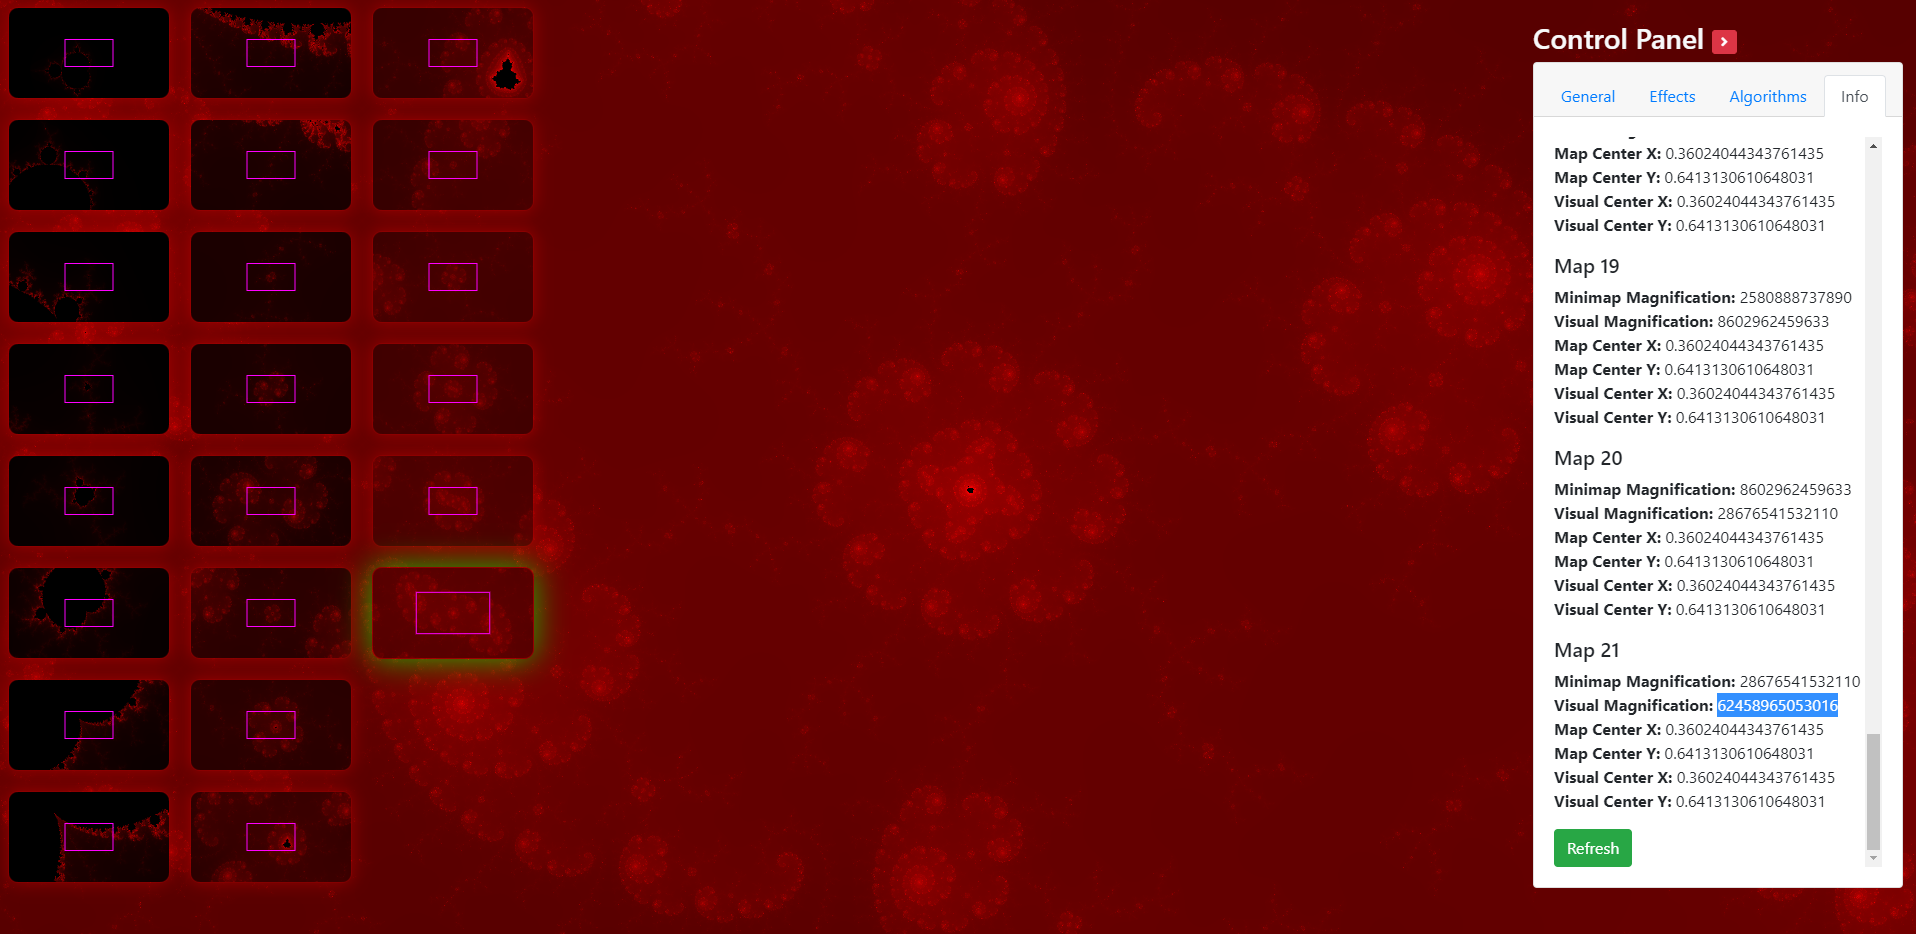
\includegraphics{Figures/Chapter5/deep.png}
\decoRule
\caption[Zooming Deep Into the Dataset]{The application can go deep into the dataset at a level of around $62$ trillions times deeper than the original, under default settings, with quite some context views occupying large portion of the visual area.}
\label{fig:chap5:deep}
\end{figure}

The basic functionalities are successfully implemented and in the following sections we'll be talking about the implementation of effects.

\subsection{Scrollbar + Dock Effect}
\label{chap5:scrollbar}

The effect \emph{Scrollbar + Dock} adds a modern-looking scrollbar on the container of the context views, making the context views not occupying too much space on the screen monitor. When user wants to browse the contexts, the scrollbar can be dragged in either directions or the mouse wheel can be used to navigate through different levels of contexts, as shown in \gmref{fig:chap5:scrollbar}.

The Apple Dock effect can also be seen clearly from the illustration that the focused context view are enlarged with its nearby contexts with lesser increment in dimensions.

\begin{figure}[H]
\centering
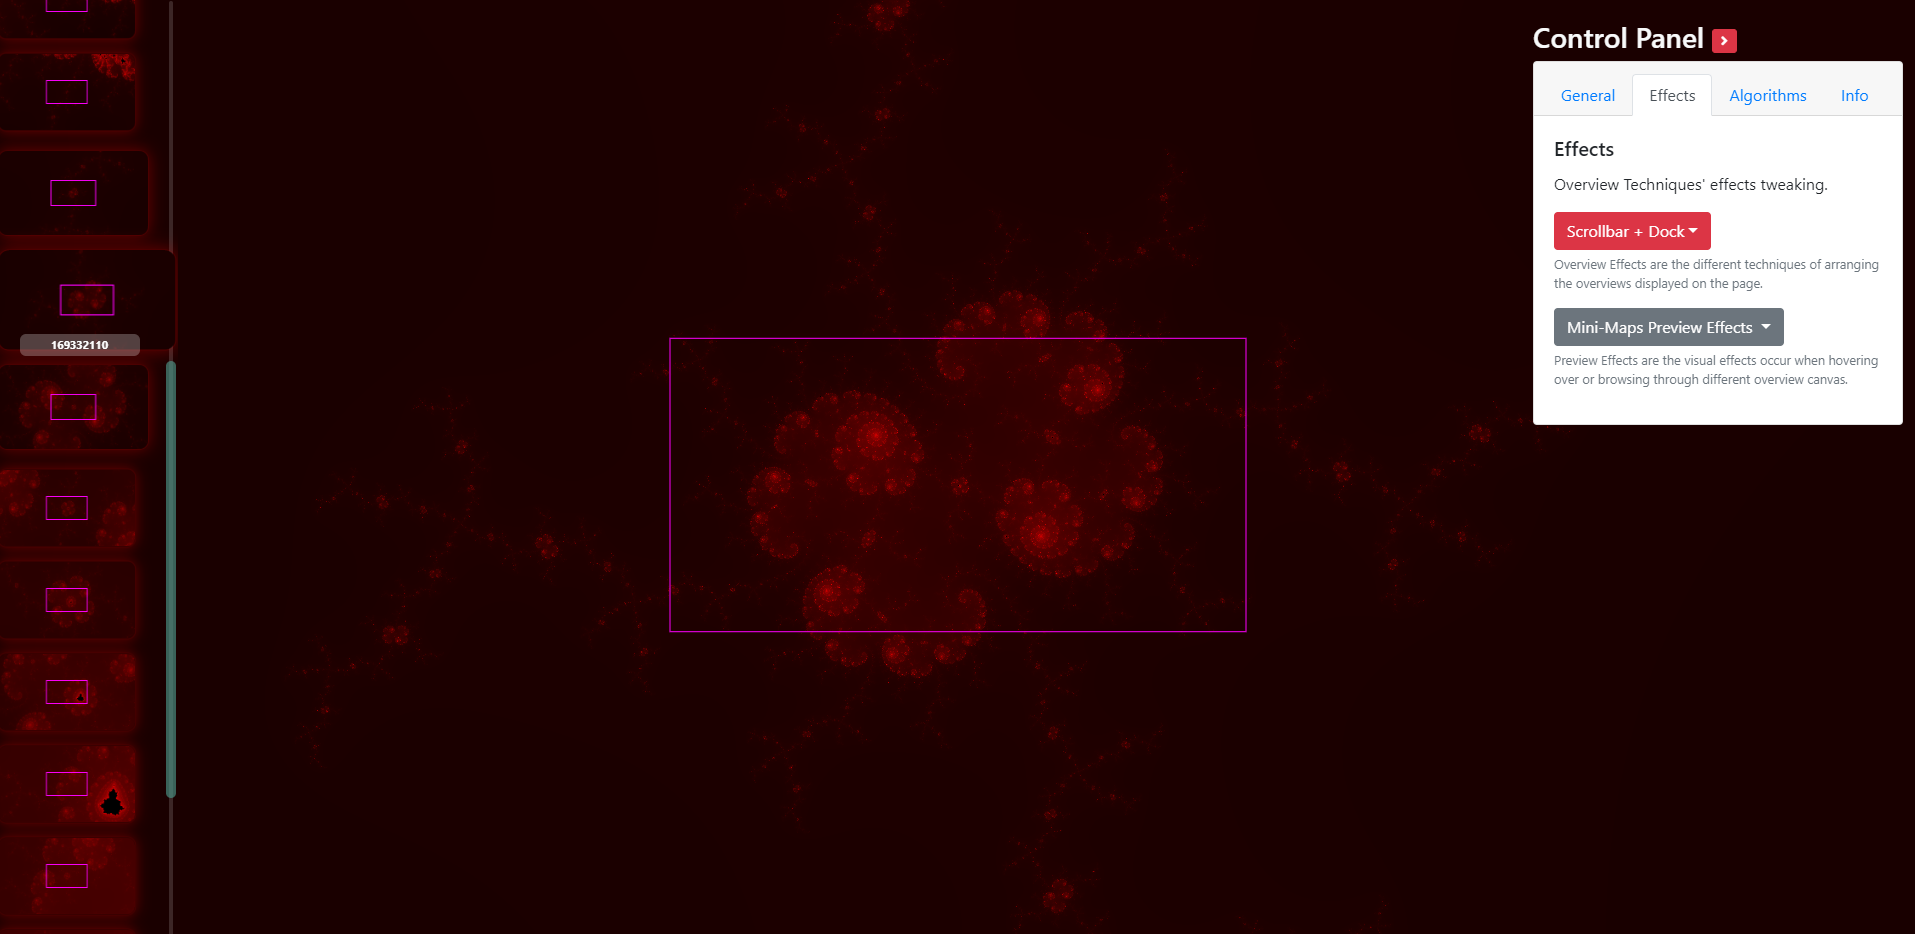
\includegraphics[width=\textwidth,keepaspectratio]{Figures/Chapter5/scrollbar.png}
% 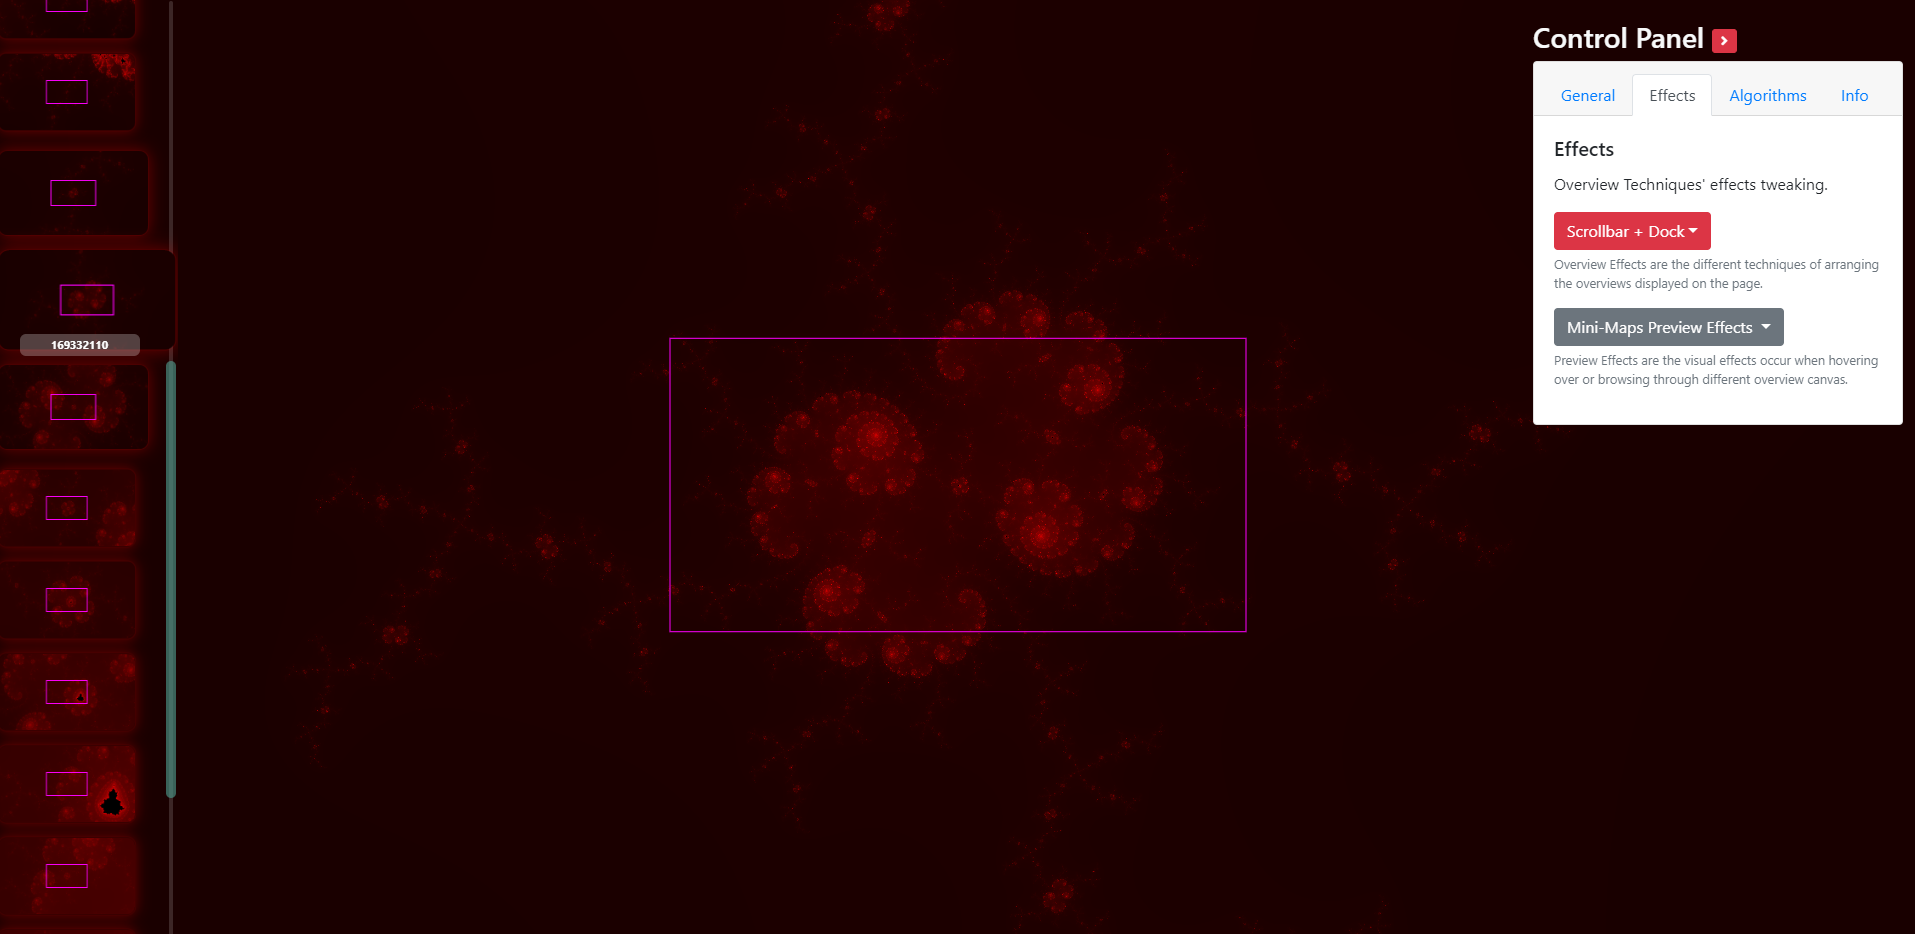
\includegraphics{Figures/Chapter5/scrollbar.png}
\decoRule
\caption[Scrollbar + Dock Effect]{A simple demonstration of the \emph{Scrollbar + Dock} effect under the magnification level of around $62$ trillions and $22$ context views.}
\label{fig:chap5:scrollbar}
\end{figure}

\subsection{Stacked Cards}
\label{chap5:cards}

The effect \emph{Stacked Cards} makes all the context views stay on one screen monitor and stack upon each other with fancy effects of rotations on the x-axis in 3d space, as shown in \gmref{fig:chap5:cards}. Note that it manages the margins between all context views nicely under the situation of the amount of context views being a relatively large number of $22$.

\begin{figure}[H]
\centering
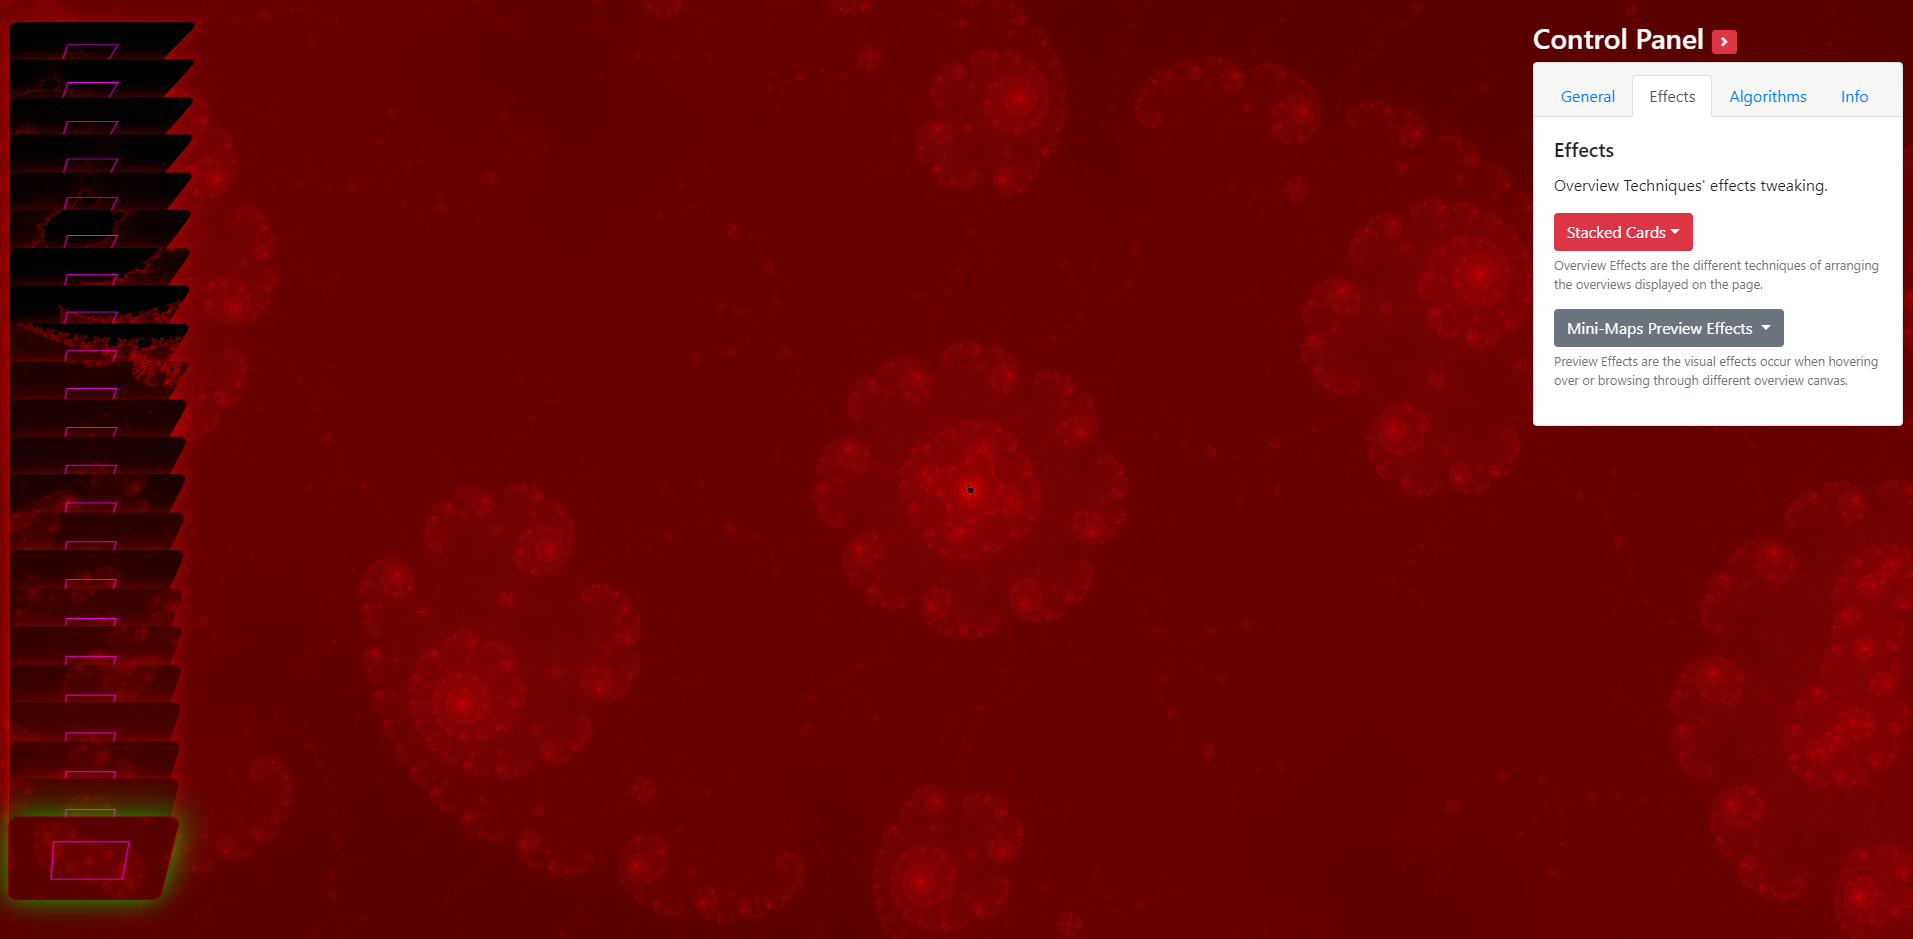
\includegraphics[width=\textwidth,keepaspectratio]{Figures/Chapter5/cards.png}
% 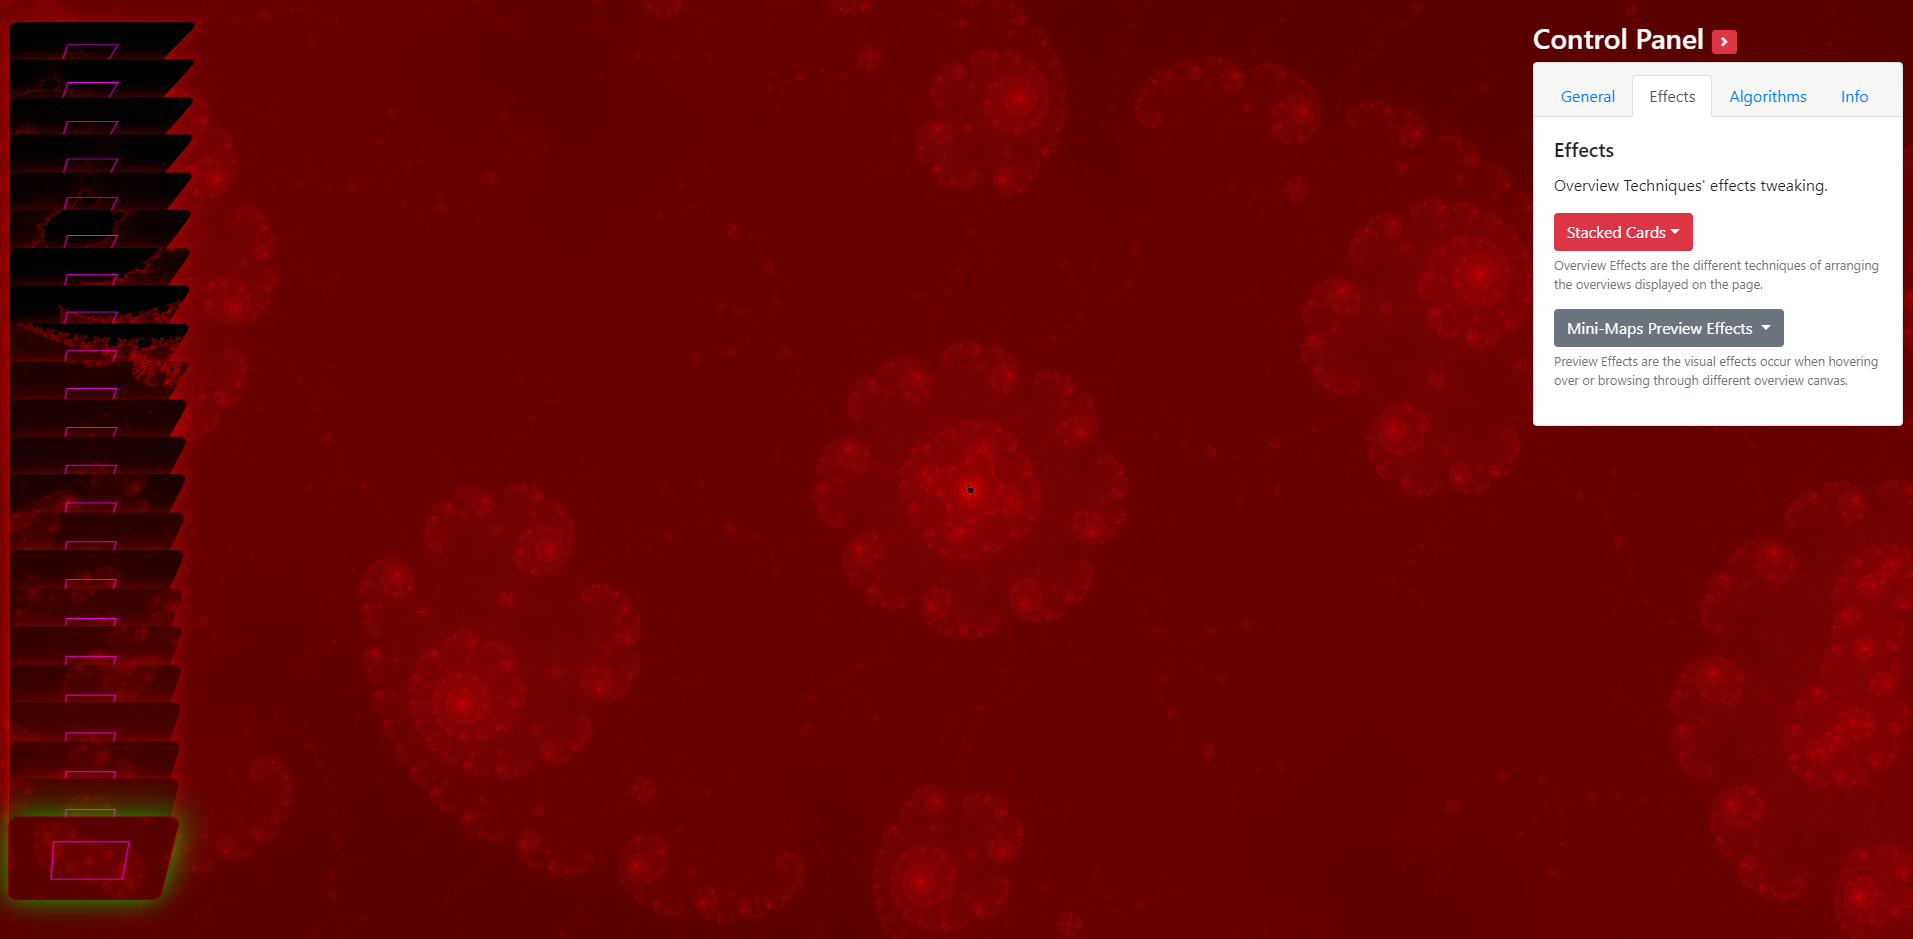
\includegraphics{Figures/Chapter5/cards.png}
\decoRule
\caption[Stacked Cards Effect]{A simple demonstration of the \emph{Stacked Cards} effect under the magnification level of around $62$ trillions and $22$ context views.}
\label{fig:chap5:cards}
\end{figure}

It is also worth mentioning that when user tries to focus one context view as shown in \gmref{fig:chap5:cards2}, that view will be emphasized by a pushing effect between itself and it's adjacent contexts with smooth 3d animations.

\begin{figure}[H]
\centering
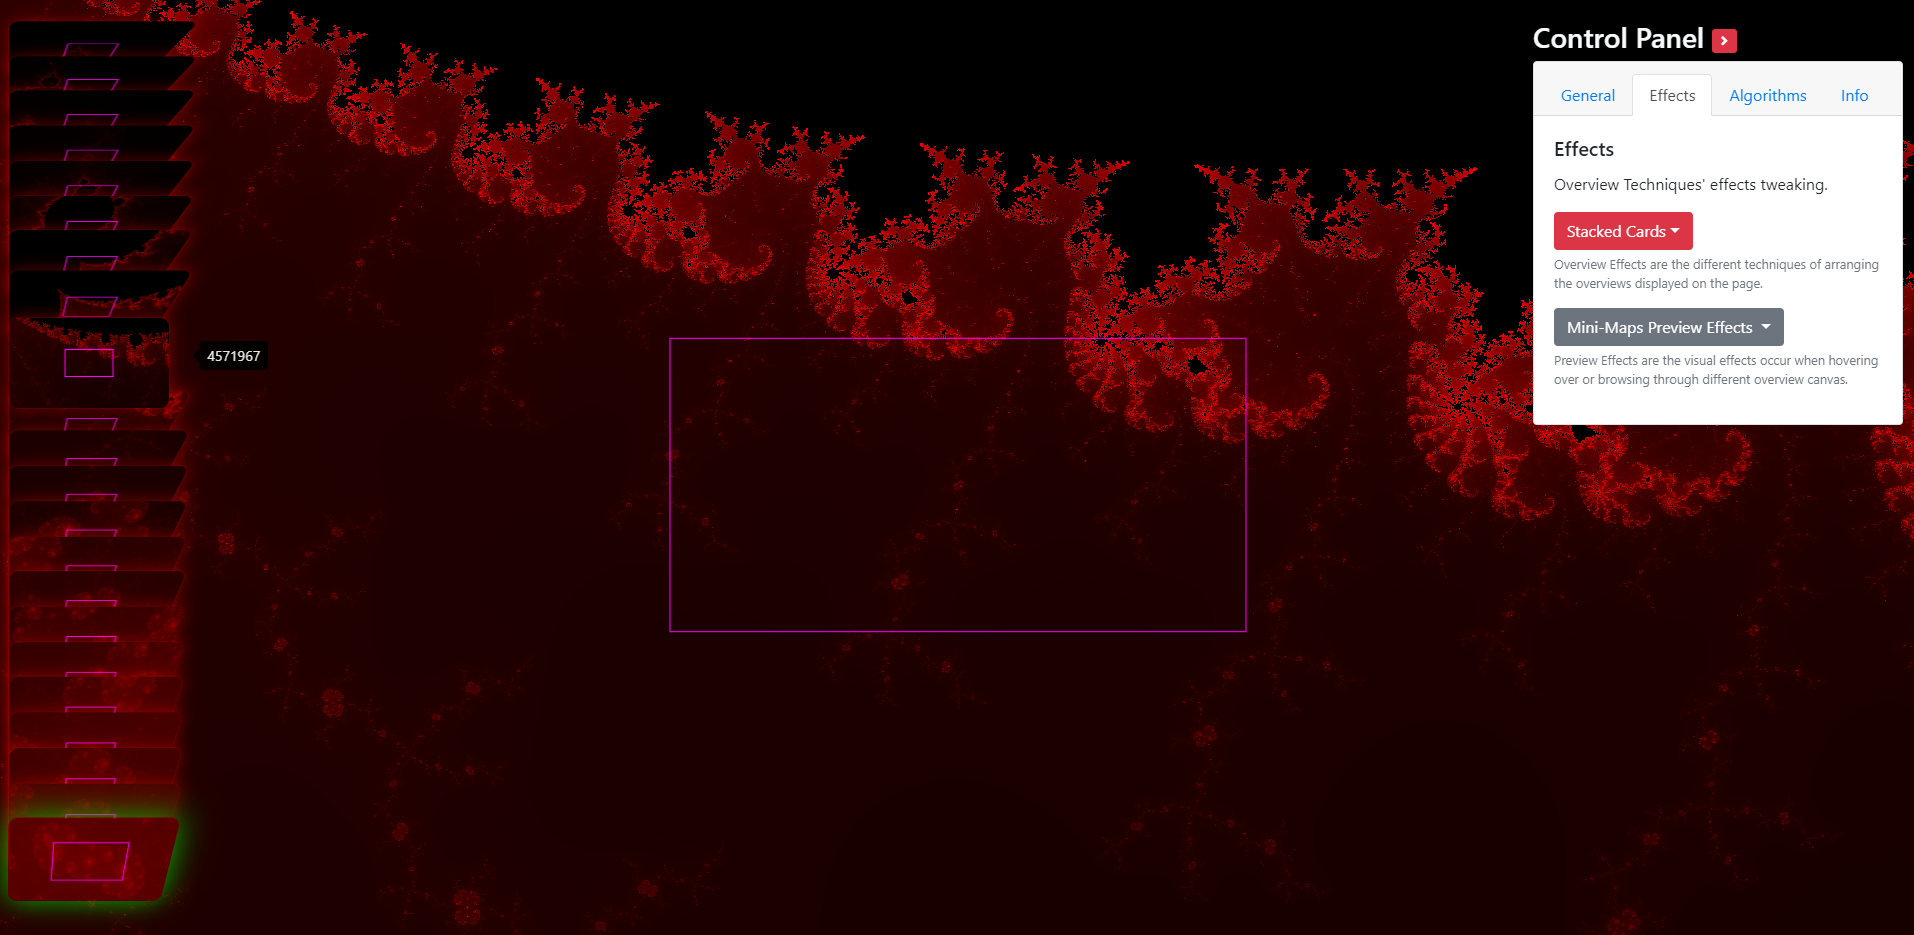
\includegraphics[width=\textwidth,keepaspectratio]{Figures/Chapter5/cards2.png}
% 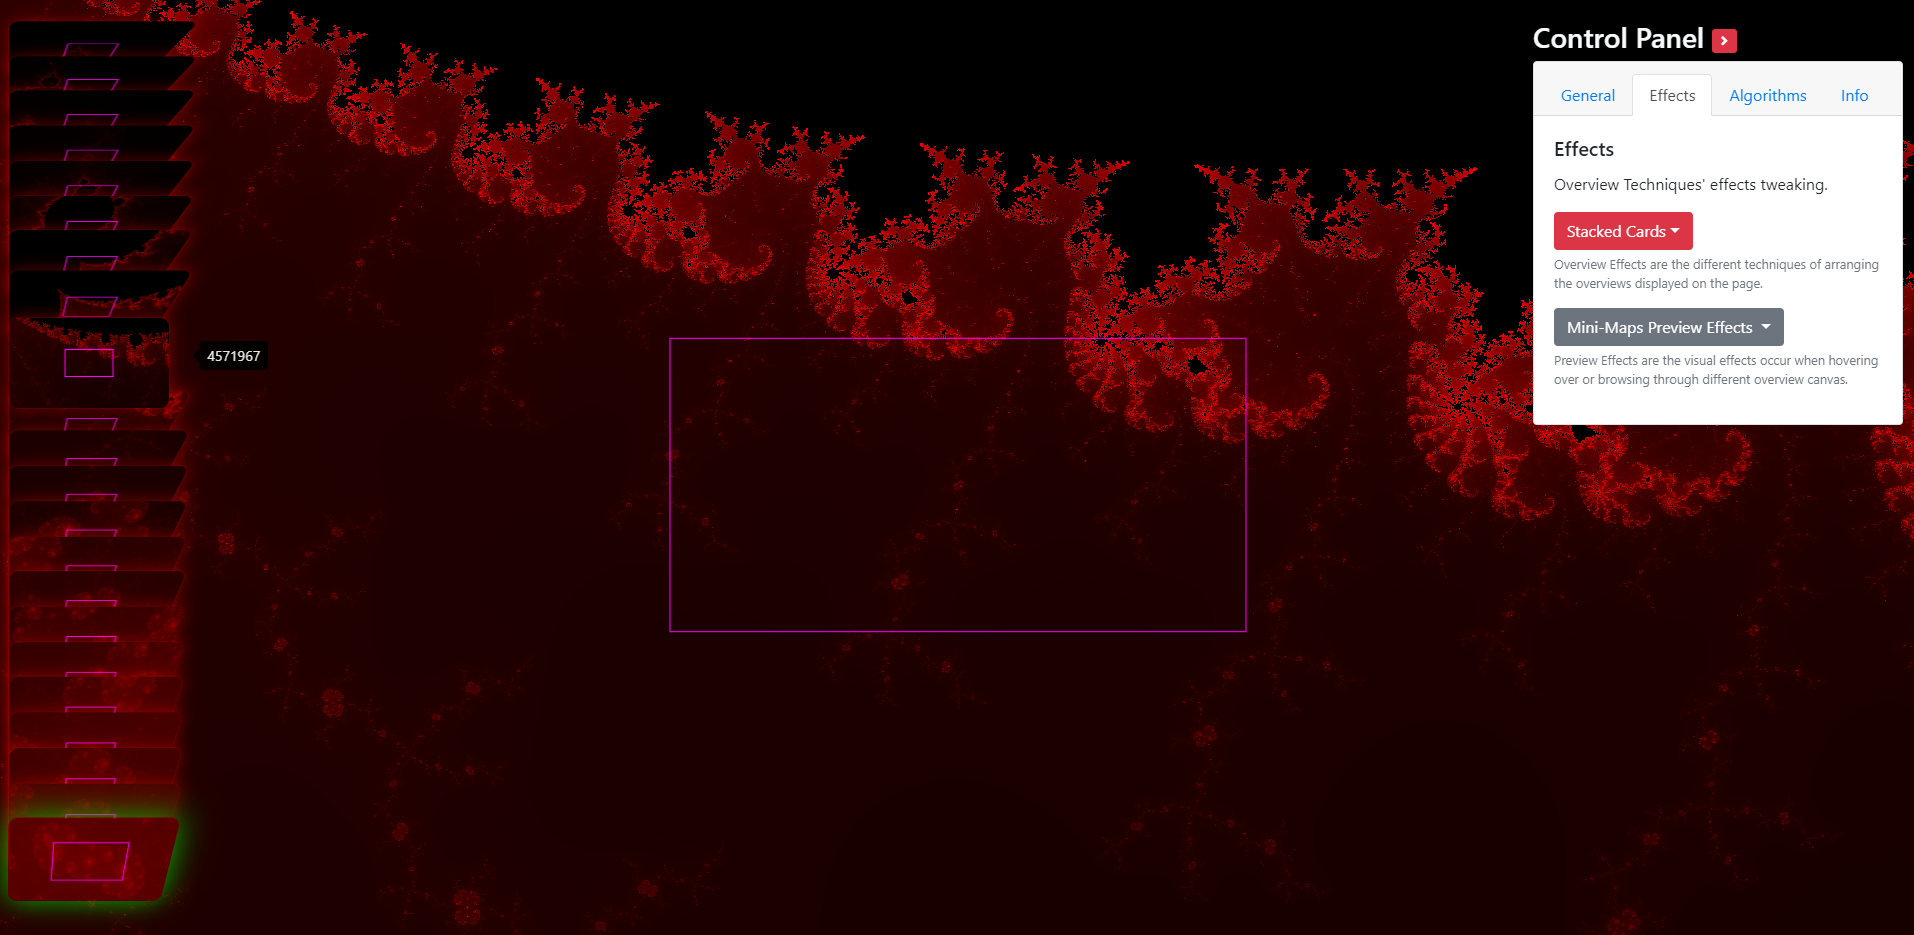
\includegraphics{Figures/Chapter5/cards2.png}
\decoRule
\caption[Stacked Cards Effect with One Focused Context View]{When one context view is focused, it ends up in a nice isolation to be emphasized amongst other views. The transition from \gmref{fig:chap5:cards} to this state is smooth with 3d rotations.}
\label{fig:chap5:cards2}
\end{figure}

\subsection{Tabs}
\label{chap5:tabs}

The effect \emph{Tabs} puts all \glspl{map} on the top side of the screen, like how modern browsers handle the open tab pages, shown in \gmref{fig:chap5:tabs}. As the number of the context views goes higher, the widths of the tabs will become smaller, like a web browser. The images of the dataset are not distorted in this arrangement and only cropped with the central data kept, as expected.

\begin{figure}[H]
\centering
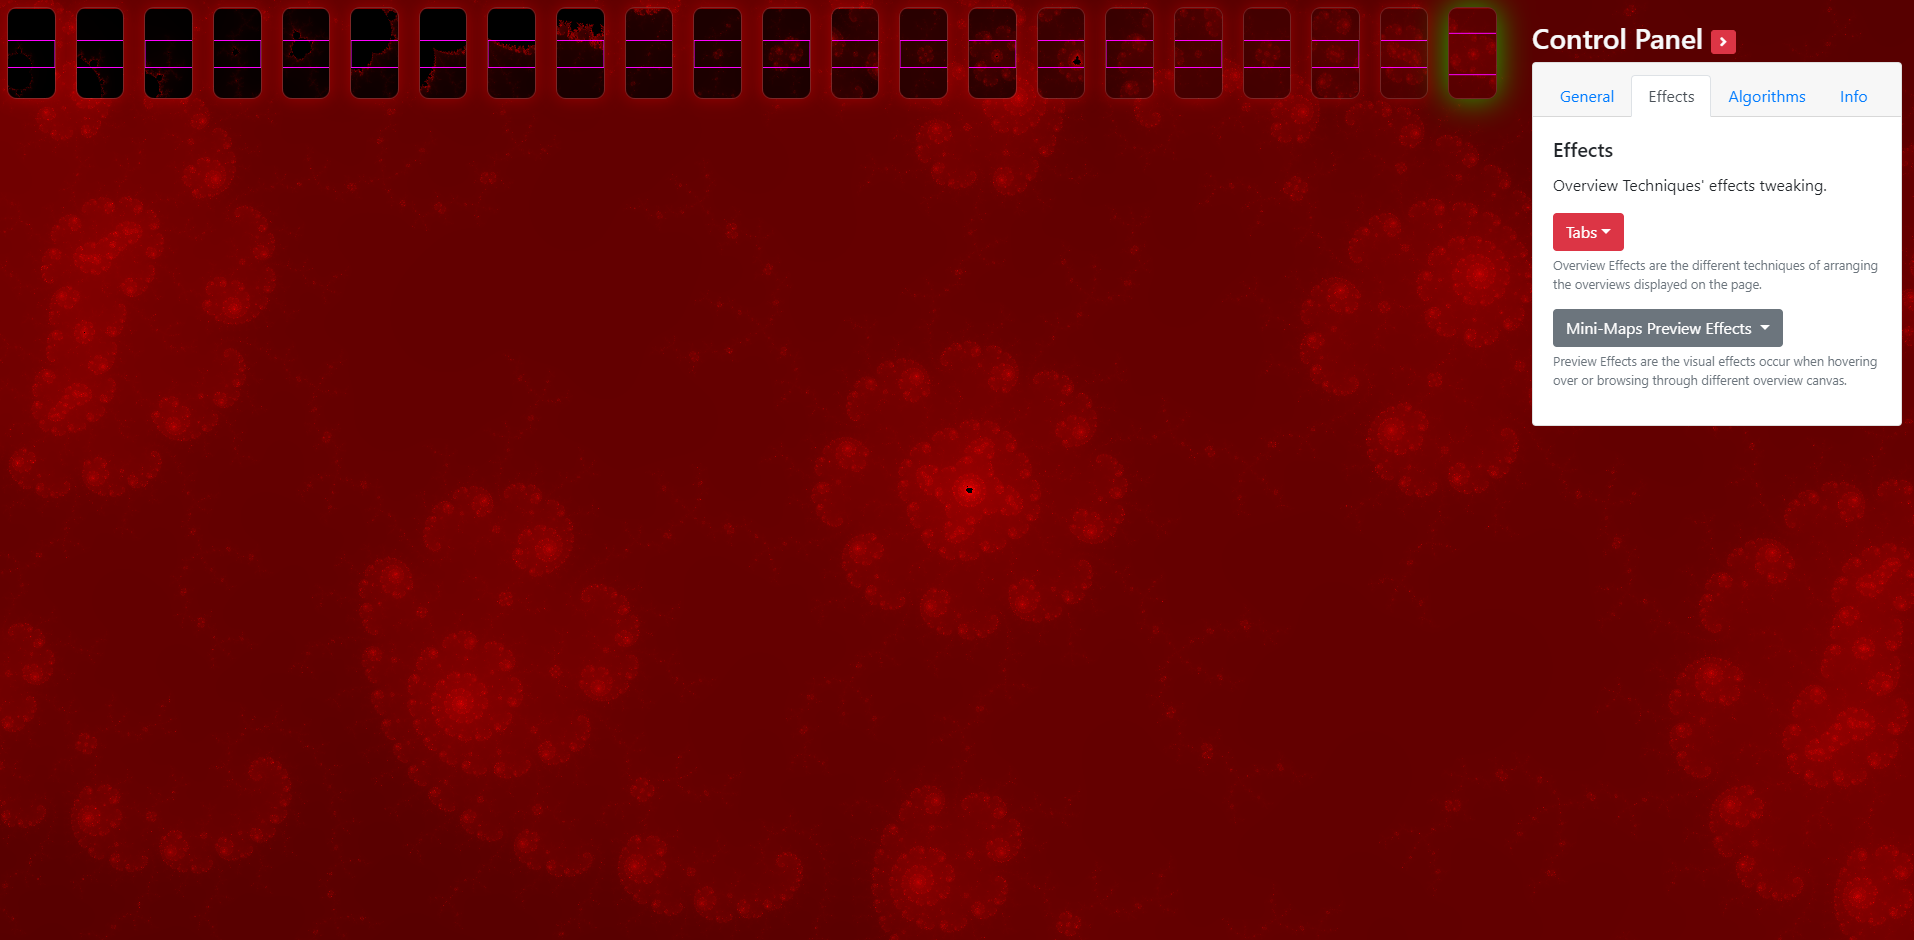
\includegraphics[width=\textwidth,keepaspectratio]{Figures/Chapter5/tabs.png}
% 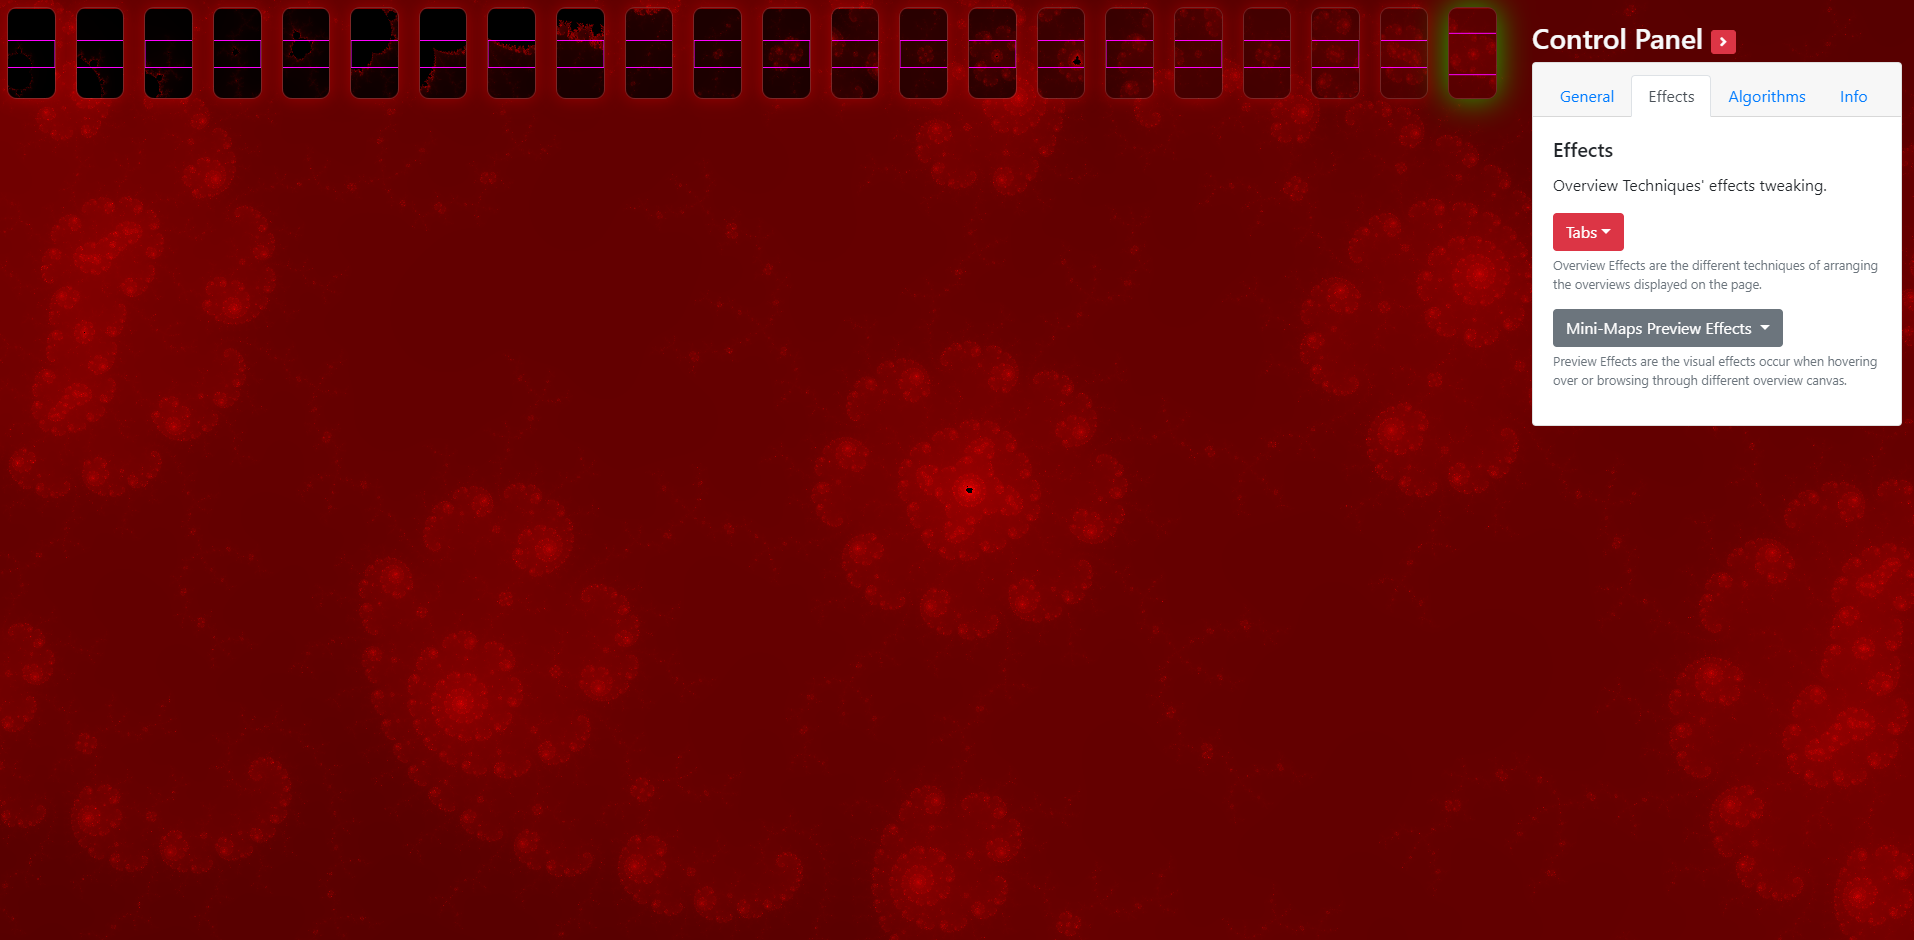
\includegraphics{Figures/Chapter5/tabs.png}
\decoRule
\caption[Tabs Effect]{A simple demonstration of the \emph{Tabs} effect under the magnification level of around $62$ trillions and $22$ context views.}
\label{fig:chap5:tabs}
\end{figure}

When a certain view is focused, as shown in \gmref{fig:chap5:tabs2}, the context view is expanded into its full form and a tooltip of the corresponding magnification level will be shown. This behaviour is as expected and is very much like how browsers treat the title of the focus tab.

\begin{figure}[H]
\centering
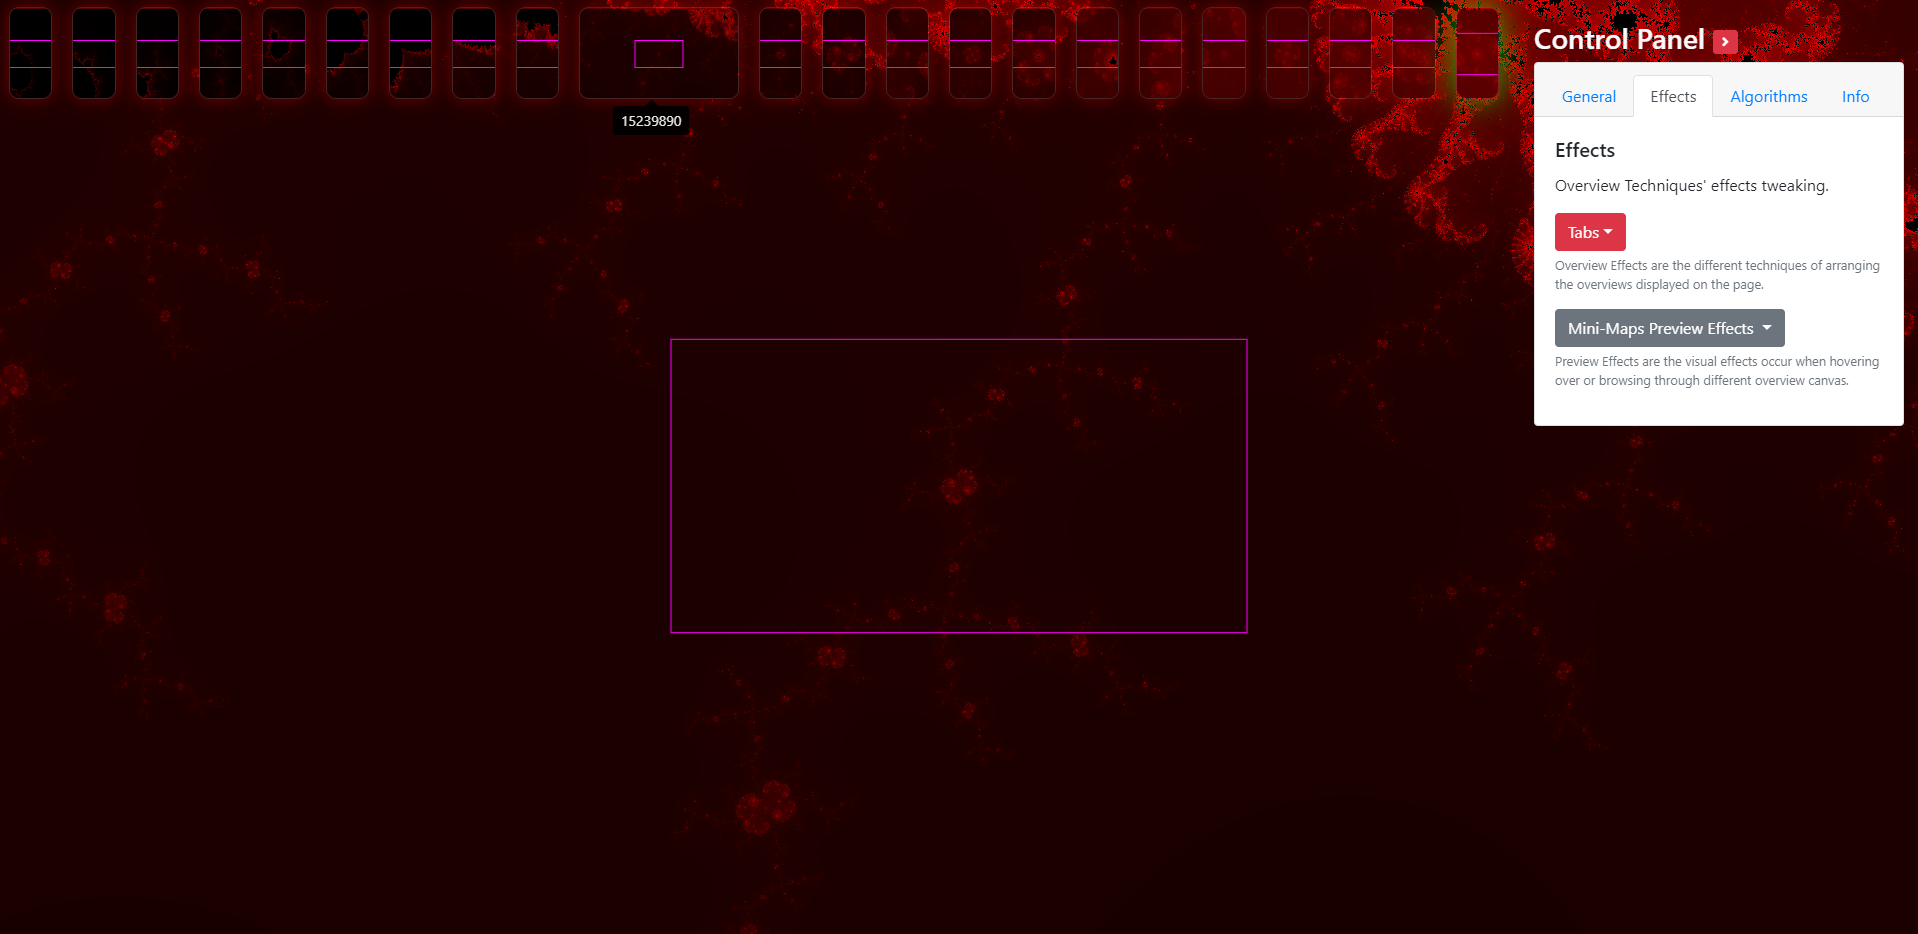
\includegraphics[width=\textwidth,keepaspectratio]{Figures/Chapter5/tabs2.png}
% 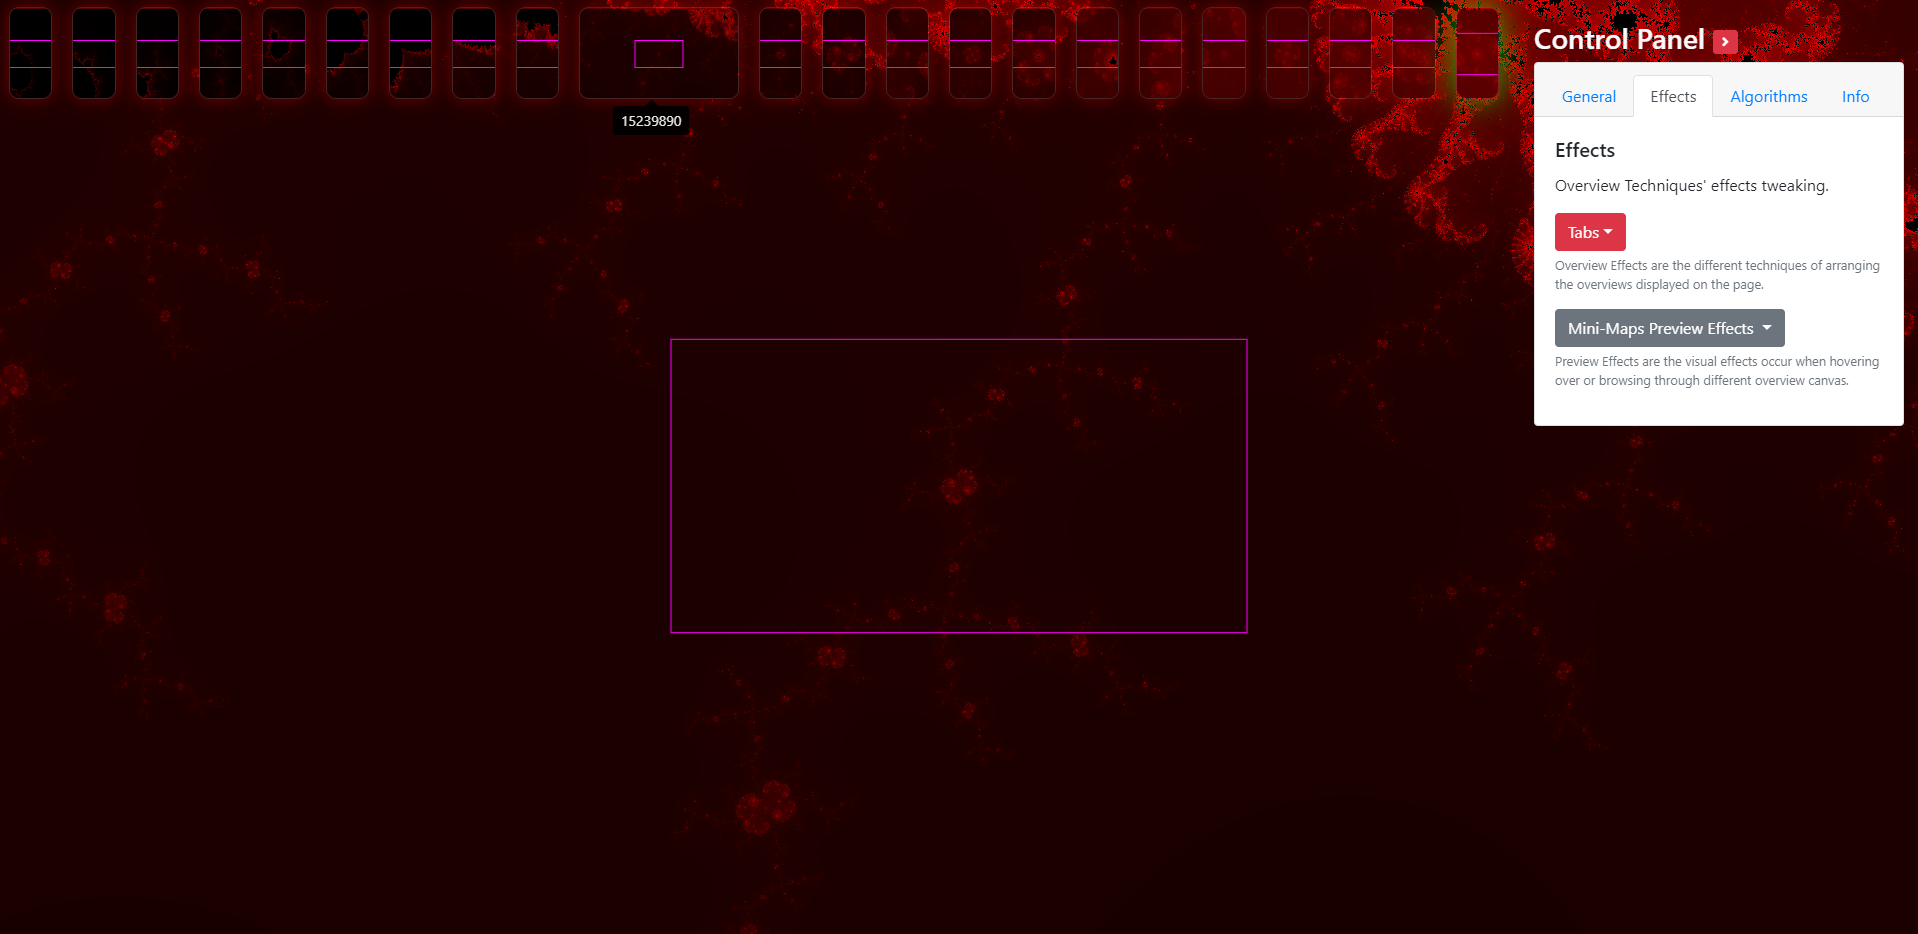
\includegraphics{Figures/Chapter5/tabs2.png}
\decoRule
\caption[Tabs Effect with One Focused Context View]{One ``tab'' is focused like how modern browsers show the complete title of the current focus web page.}
\label{fig:chap5:tabs2}
\end{figure}

As all the above \gls{map} effects have been verified success, we'll be talking about the preview effects of the context views.

\subsection{Fade In / Out Preview Effect}
\label{chap5:fade}

The \emph{Fade In / Out} preview effect applies a fade-in and a fade-out effect for the display of \gls{fhd} version of the context views, as shown in \gmref{fig:chap5:fadepreview}, preventing the presentation of the context view from being too abrupt.

\begin{figure}[H]
\centering
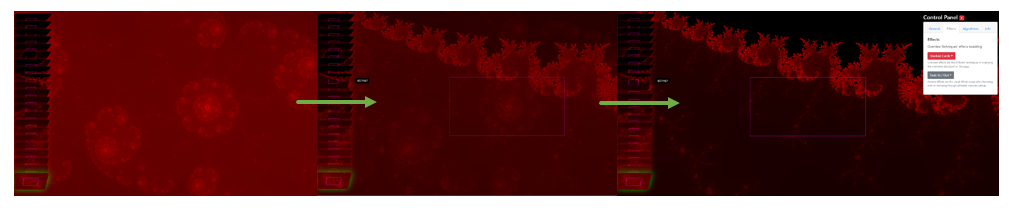
\includegraphics[width=\textwidth,keepaspectratio]{Figures/Chapter5/fadepreview.png}
% 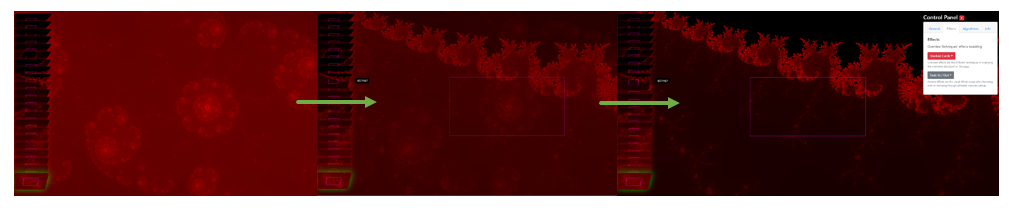
\includegraphics{Figures/Chapter5/fadepreview.png}
\decoRule
\caption[Fade In / Out Preview Effect]{Animation of the \emph{Fade In / Out} preview effect.}
\label{fig:chap5:fadepreview}
\end{figure}

\subsection{Zooming Through Preview Effect}
\label{chap5:zoom}

The \emph{Zooming Through} preview effect applies a smooth animation on the activation of the focus of one context. Once a context view is focused, instead of directly showing the \gls{fhd} version of the context view, a zooming animation is taken place until the zoom reaches the desired context view from the previous context or detail view, in a sense of depths, as shown in \gmref{fig:chap5:zoompreview}.

\begin{figure}[H]
\centering
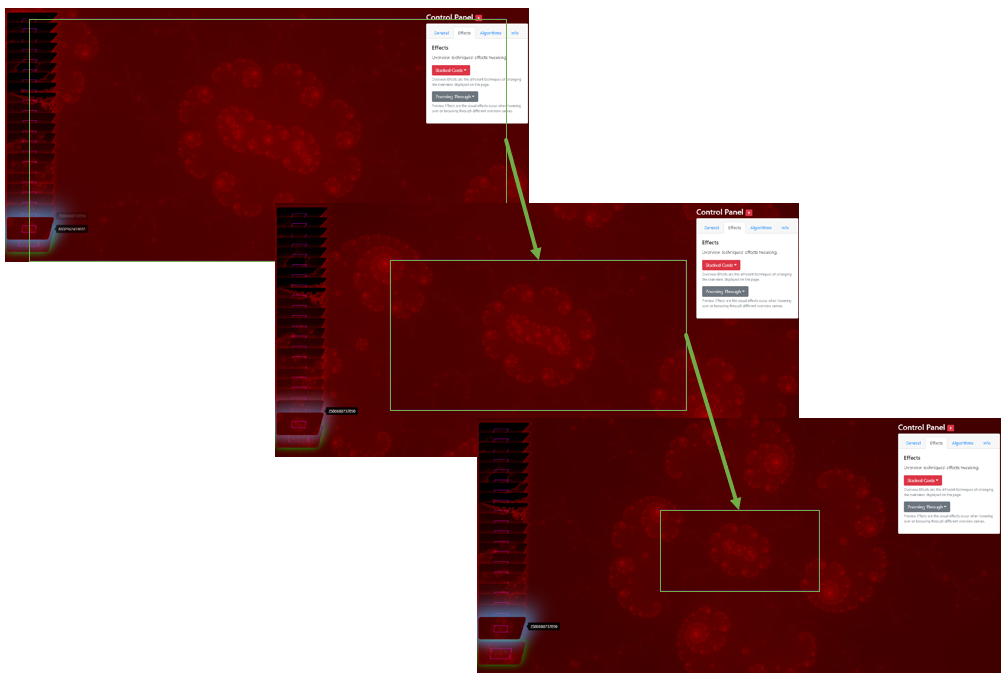
\includegraphics[width=\textwidth,keepaspectratio]{Figures/Chapter5/zoompreview.png}
% 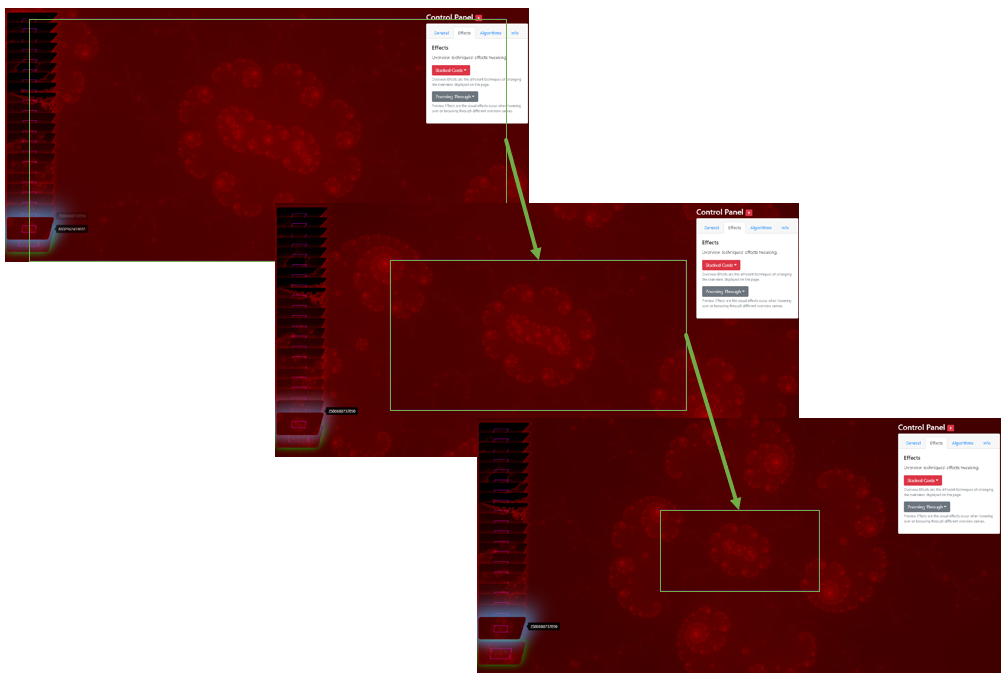
\includegraphics{Figures/Chapter5/zoompreview.png}
\decoRule
\caption[Zooming Through Preview Effect]{Animation of the \emph{Zooming Through} preview effect.}
\label{fig:chap5:zoompreview}
\end{figure}

%----------------------------------------------------------------------------------------
%	SECTION
%----------------------------------------------------------------------------------------

\section{Comparison Between Different Overview Techniques}

In this section, we'll be analyzing and compare the different overview techniques that are implemented in this project.

In the aspect of functionalities, we introduced the following two different types of techniques:

\begin{itemize}
    \item Overview Arrangement Effects
    \item Preview Effects
\end{itemize}

The differences are shown in \gmref{tbl:types}.

\begingroup
\centering
\begin{tabu} to .97\textwidth { | X[1, r, m] | X[3, l, m] | }
    \hline
    Type & Functionality \\
    \hline\hline
    Overview Arrangement Effects &
    \vspace{.85em}\begin{itemize}
        \item Gives the hierachical structure
        \item The arrangements of the overviews
    \end{itemize} \\
    \hline
    Preview Effects &
    \vspace{.85em}\begin{itemize}
        \item The preview effects of the overview
        \item Transition between the different preview display
    \end{itemize} \\
    \hline
\end{tabu}
\captionof{table}{Different Types of Techniques}\label{tbl:types}
\endgroup

In the following sections, we'll be comparing these two types of overview techniques respectively. In turn, we'll be comparing them in the following aspects:

\begin{itemize}
    \item Characteristics in dataset expression(expressiveness)
    \item Applicable situations
\end{itemize}

The aspect ``characteristics in dataset expression'' can be shortened in the following sections as \emph{expressiveness}.

\subsection{Overview Arrangement Effects}

We designed and realized three ways of overview arrangements effects:

\begin{itemize}
    \item \emph{Scrollbar + Dock} overview arrangements effect, described in \gmref{chap5:scrollbar}
    \item \emph{Stacked Cards} overview arrangements effect, described in \gmref{chap5:cards}
    \item \emph{Tabs} overview arrangements effect, described in \gmref{chap5:tabs}
\end{itemize}

Including the settings of when no effects are applied, there are in total four different ways of arranging the overviews. The situation when no management is applied to the overviews can be considered as a reference to be compared with, which is a situation when the problems were not solved before this project.

The effect \emph{Scrollbar + Dock} adds a modern-looking scrollbar to the list of overviews, making them only occupying a fixed amount of space on the screen monitor. When user wants to browse through the different depths of the index of the overviews, the scrollbar can be dragged in either directions or the mouse wheel can be used to navigate through different levels of overviews. The Dock effect emphasizes the focused overview by different enlargement and margins applied on the overviews.

The effect \emph{Stacked Cards} distributes all the overviews on the left side of the screen monitor with rotations on the x-axis of the virtual 3d space on the web page. It manages the margins between all overviews nicely and spread them with equal amount or margins between them. When user tries to focus one overview, it levitates the overview on the most top level and rotate it back to initial state in 3d space, and isolates it from other overviews with a larger margins.

The effect \emph{Tabs} distributes all overviews on the top side of the screen evenly, and does necessary adjustment on their widths to make them all fit. The adjustment performed are cropping actions to display only the key information, the information around the center, of each overviews. When a certain view is focused, it is restored to its orignal form and a tooltip of the corresponding magnification level will be shown.

The characteristics in dataset expression for all these overview arrangement effects are shown in \gmref{tbl:overview:exp}.

\begingroup
\centering
\begin{tabu} to .97\textwidth { | X[1, r, m] | X[3, l, m] | }
    \hline
    Type & Characteristics in Dataset Expression \\
    \hline\hline
    \emph{Scrollbar + Dock} &
    \vspace{.85em}\begin{itemize}
        \item Tidy and clean visual effects in sense of expression
        \item Modern looking scrollbar that induces comfort when browsing through the depths of data
        \item Focused overview have strong visual emphasized effects, as the adjacent overviews serve as foils with a lesser enlargement level
        \item Overviews have their original aspect ratios kept, not distorted, with all information presented if on screen
        \item Controls over the index of overviews are extremely intuitive using scrollbar as navigator
    \end{itemize} \\
    \hline
    \emph{Stacked Cards} &
    \vspace{.85em}\begin{itemize}
        \item Impactful and gorgeous appearance with great amount of tensions
        \item 3d designs making depths of dataset more vivid and intuitive
        \item Strong designs for focused overview that separates it from other overviews
        \item Fascinating 3d transitions induce sensory enjoyment when the ``cards'' are flipping
        \item Modern looking tooltips that show exactly the information that are interested, the magnification level
        \item Expressing all depths of overview data within one single screen
    \end{itemize} \\
    \hline
    \emph{Tabs} &
    \vspace{.85em}\begin{itemize}
        \item Tidy and clean visual effects in sense of expression
        \item Simple tab designs that induces senses of classiness
        \item Focused overview have strong visual emphasized effects, as it is transitioned into its full form with all information presented
        \item Although overviews don't have all of their original information presented within one single screen, however, their aspect ratios are kept and key information are presented, as the presented overviews are only cropped off with the information around the left and right edges
        \item Modern looking tooltips that show exactly the information that are interested, the magnification level
        \item Controls over the index of overviews are extremely intuitive using the conventional ways of tab arrangement of modern browsers
        \item Expressing all depths of overview data within one single screen, holding even more than the effect \emph{Stacked Cards}
    \end{itemize} \\
    \hline
    No effects &
    \vspace{.85em}\begin{itemize}
        \item Tidy and clean appearance
        \item Conventional arrangement
    \end{itemize} \\
    \hline
\end{tabu}
\captionof{table}{Expressiveness for Overview Arrangements}\label{tbl:overview:exp}
\endgroup

The applicable situations for all the mentioned overview arrangement effects are shown in \gmref{tbl:overview:app}.

\begingroup
\centering
\begin{tabu} to .97\textwidth { | X[1, r, m] | X[3, l, m] | }
    \hline
    Type & Applicable Situations \\
    \hline\hline
    \emph{Scrollbar + Dock} &
    \vspace{.85em}\begin{itemize}
        \item When intuive controls over the index of overviews are needed, since scrollbar is an intuive concept of browsing through larger amount of data
        \item When a portion of a larger amount of overviews are to be focused, since the scrollbar makes the viewport displaying a part of the layers of the overviews only, indicating them to be focused
        \item When more focus are needed in general, as the Dock effect induces
    \end{itemize} \\
    \hline
    \emph{Stacked Cards} &
    \vspace{.85em}\begin{itemize}
        \item When a sense of high tech is needed for the presentation of the dataset, since 3d animations are modern-looking with great amount of tensions
        \item When all overviews are needed to be presented within one screen monitor, as it has the capability of holding all overviews within one screen
        \item When great depths of the index of all the overviews are needed to be presented, as it offers a sense to the user a vast range of depths of overviews through the 3d arrangement
    \end{itemize} \\
    \hline
    \emph{Tabs} &
    \vspace{.85em}\begin{itemize}
        \item When a sense of classiness is needed for the presentation of the dataset, since designs of \emph{Tabs} is elegant
        \item When all overviews are needed to be presented within one screen monitor, as it has the capability of holding all overviews within one screen
        \item When great depths of the index of all the overviews are needed to be presented in a straightforward and less fancy way, as it puts all the overviews lined up with key information
    \end{itemize} \\
    \hline
    No effects & 
    \vspace{.85em}\begin{itemize}
        \item When simple requirements are to be fulfilled, as it includes all basic functionalities
    \end{itemize} \\
    \hline
\end{tabu}
\captionof{table}{Applicable Situations for Overview Arrangements}\label{tbl:overview:app}
\endgroup

\subsection{Preview Effects}

We designed and realized two ways of preview effects:

\begin{itemize}
    \item \emph{Fade In / Out} preview effect, described in \gmref{chap5:fade}
    \item \emph{Zooming Through} preview effect, described in \gmref{chap5:zoom}
\end{itemize}

Including the settings of when no effects are applied, there are in total three different ways of previewing an overview. 

The \emph{Fade In / Out} preview effect applies a transition on the transparency of between the current viewing area, either the detail view or the preview of another overview, and the overview to be previewed, preventing the preview of the \gls{fhd} version of the overview from being too abrupt.

The \emph{Zooming Through} preview effect applies a smooth animation of the traveling process from one certain depth of overview to another, instead of directly showing the \gls{fhd} version of the preview of the desired overview. The traveling process is presented in a zooming fashion in a sense of depths.

The characteristics in dataset expression for all these preview effects are shown in \gmref{tbl:preview:exp}.

\begingroup
\centering
\begin{tabu} to .97\textwidth { | X[1, r, m] | X[3, l, m] | }
    \hline
    Type & Characteristics in Dataset Expression \\
    \hline\hline
    \emph{Fade In / Out} &
    \vspace{.85em}\begin{itemize}
        \item Mild and gentle transitions when switching between different previews, displaying and hiding previews
        \item Induces comfort and not being abrupt for users when trying to preview
        \item Proper duration of the animations
    \end{itemize} \\
    \hline
    \emph{Zooming Through} &
    \vspace{.85em}\begin{itemize}
        \item Dramatic visual effects with great amount of tensions, like in the movies
        \item The sense of depths of the overviews becomes extremely strong, as it travels through all the depths on the way of ``sinking'' or ``levitating''
        \item Animations designed making the transition impactful at the same time progressive
    \end{itemize} \\
    \hline
    No effects &
    \vspace{.85em}\begin{itemize}
        \item Take immediate effect of previewing a certain overview
        \item Zero time left for animations
    \end{itemize} \\
    \hline
\end{tabu}
\captionof{table}{Expressiveness for Preview Effects}\label{tbl:preview:exp}
\endgroup

The applicable situations for all the mentioned preview effects are shown in \gmref{tbl:preview:app}.

\begingroup
\centering
\begin{tabu} to .97\textwidth { | X[1, r, m] | X[3, l, m] | }
    \hline
    Type & Applicable Situations \\
    \hline\hline
    \emph{Fade In / Out} &
    \vspace{.85em}\begin{itemize}
        \item When the situation of only separate overviews need to be previewed and the connections between them are not as important
        \item When smooth transitions are needed or trying to avoid the preview process of being abrupt
        \item When short animation time can be applied to the presentation of the dataset
    \end{itemize} \\
    \hline
    \emph{Zooming Through} &
    \vspace{.85em}\begin{itemize}
        \item When the sense of depths are essential or the connections between different levels of overviews should be emphasized, as all the preview process gives the traveling animations
        \item When longer animation can be applied to the presentation of the dataset
    \end{itemize} \\
    \hline
    No effects &
    \vspace{.85em}\begin{itemize}
        \item When the situation of only separate overviews need to be previewed and the connections between them are not as important
        \item The importance of immediate previews are needed, since it doesn't have any animations and previews are instantly shown
    \end{itemize} \\
    \hline
\end{tabu}
\captionof{table}{Applicable Situations for Preview Effects}\label{tbl:preview:app}
\endgroup

\subsection{Other Aspects}

In the aspect of performance, all overview arrangement effects as well as the preview effects are flashy fast and doesn't induce higher cost for hardwares. One click selection from the dropdown menu will have corresponding effects taken place immediately.

Parameters control of all the effects are intuitive and simple on the same level, as they are all one click away. All necessary parameters offer enough controls over them. 

As for the implementation, since the project is following a same pattern as described before, the codes of this project is extremely readable and maintainable. New effects can be implemented and plugged in easily following the same pattern as described. The resolver can also be easily replaced and adapted by some other forms of it, as long as it can solve the same problem and taking similar parameters.

%----------------------------------------------------------------------------------------
%	SECTION
%----------------------------------------------------------------------------------------

\section{Future Work}

For future work that can be done on this project:

\begin{itemize}
    \item More advanced calculation on the back end side, for example implement perturbation techniques\footnote{ For info can be found at \url{https://mathr.co.uk/mandelbrot/perturbation.pdf} at the time this thesis is composed.} or \emph{SuperFractalThing}\footnote{ Check \url{http://www.chillheimer.de/kallesfraktaler/} for more information} algorithms to improve the capabilities of deep zooming for this project.
    \item Use other languages other than script languages such as \emph{Python} with math enhancement libraries or \emph{C++} based lower level languages to improve speed of calculation. Other algorithms could also be implementd.
    \item Replace the back end resolver from a multi-threading script with a real server responder. The previous two improvements can be combined with this one.
    \item More detailed control panel can be implemented, giving more control over this project.
    \item More visual effects, overview management effects and preview effects can be done following the same patterns that this project has created and followed.
\end{itemize}

To think even wider:

\begin{itemize}
    \item Replace the back end from the calculation of a mathematical dataset with real world dataset, such as \gls{gis} data.
    \item Enhance the coordination system from simple 2d Cartesian system to curvilinear coordinates that can suit the above needs.
    \item Projection of the focus area calculated can be levitated from strict rectangles to quadrilaterals when the dataset being observed becomes 3d.
\end{itemize}